\documentclass[english,a4paper,12pt]{report}
\usepackage{mypackage}

\title{Electrodynamics}

\author{Haydn Cheng}

\date{\today}

\begin{document}
\maketitle
\tableofcontents
    
\chapter{Electrostatics}

Electrostatics is the study of the interactions between charged particles that are stationary.\footnote{Actually, it is not necessary that the charges be stationary, but only that the charge dneisy at each poitn be constat. For example, a rotating sphere with uniform charge density produce an electrostatic field \(\displaystyle \frac{1}{4\pi \epsilon_0 r^2}\vu{r}  \), even though the charges are moving.} 

\section{Electric Fields and Potentials}

\todo{problem 1.16, 1.39} 

By the Coloumb's law, the electric field at position \(\vb{r} \) created by the volume charge density \(\rho (r')\) is

\begin{equation}
    \vb{E}(  \vb{r}) = \frac{1}{4\pi \epsilon_0} \int \frac{\rho ( \vb{r}' ) \hrcurs}{\rcurs ^2}   d\tau ', \label{comb} 
\end{equation}

where \(\brcurs = \rcurs \hrcurs = \vb{r} -\vb{r} '\) is the vector pointing from the source charge to an arbitrary point in space.

Taking the divergence, we have 

\begin{equation}
    \div{\vb{E}(\vb{r} )} = \frac{1}{4\pi\epsilon_0} \int \rho (\vb{r} ') \left(\div{\frac{\hrcurs }{\rcurs ^2} }\right) d\tau ' = \frac{1}{4\pi \epsilon_0} \int 4\pi \delta ^3 (\vb{r} - \vb{r} ')\rho (\vb{r} ') d\tau = \frac{\rho (\vb{r} )}{\epsilon _0}.  	 
\end{equation}

Taking the curl, we have 

\begin{equation}
    \curl{\vb{E}(\vb{r} ) } = \frac{1}{4\pi \epsilon_0} \int \rho(\vb{r} ') \left( \curl{ \frac{\hrcurs }{\rcurs ^2}  }\right)  d\tau'  = 0.
\end{equation}

Here \(\rho (\vb{r} ') d \tau '\) is taken out of the curl since they do not depend on \(\vb{r} \) but \(\vb{r} '\).    

These are the two Maxwell's equations under electrostatics assumptions.

We can thus define the elctric field as the (negative) gradient of a scalar function \(V(\vb{r}) \) which we call it as electric scalar potential defined by

\begin{equation}
    E(\vb{r} ) = -\grad{V(\vb{r} )}
\end{equation}

as the curl of a gradient is always zero. 

Integrating both sides,

\begin{equation}
    - \int_{\vb{a} }^{\vb{b} } \vb{E} (\vb{r} ) \cdot d\vb{r} = -\int_{\mathcal{O}}^{\vb{b} }\vb{E} \cdot d\vb{r} - \left( - \int_{\mathcal{O}}^{\vb{a} }\vb{E} \cdot d\vb{r}    \right) = \int_{\vb{a} }^{\vb{b} } \left( \grad{\vb{V} (\vb{r} )}  \right) \cdot d \vb{r}  = V(\vb{b} ) - \vb{V} (a)   
\end{equation}

Since \(\vb{a} \text { and } \vb{b} \) are arbitrary, the term that depends on \(\vb{a} \) on LHS must be equals to the term that depends on \(\vb{a} \) on RHS (and the same holds for \(\vb{b} \)). Therefore we haeve 

\begin{equation}
    V(\vb{r} ) = - \int_{\mathcal{O}}^{\vb{r} } \vb{E} \cdot d\vb{r}   
\end{equation}

Usually, the reference point \(\mathcal{O}\) is taken to be infinity, in which \(V = 0\) since it is away from all the charges.

According to the Helmoholtz theorem proved in the calculus notes, the potential can also be written as 

\begin{equation}
    V(\vb{r} ) = \frac{1}{4\pi \epsilon_0} \int \frac{\rho (\vb{r} ')}{\rcurs }d\tau ' + C \label{potential} 
\end{equation}

where \(C\) can be any constant scalar function independent of \(\vb{r} \)  which we conveniently take it as zero. Since the gradient of a constant scalar function is always zero, so the introduction of \(C\) does not affect the electric field. 

However, this form assumes that \(\vb{E} (\vb{r} )\) goes to zero as \(r \to \infty\), which is not true for charge distribution that extends to infinity such as a infinitely long wire. In those cases, we must revert back to the line integral of \(\vb{E} (\vb{r} )\) and define another reference point \(\mathcal{O}\) to calculate its potential.     

The relations between charge, electric potential and electric field is shown in \cref{elecrelations}. 

\onefig{elecrelations}{scale=0.3}

One can see that there are two ways to calculate the potential or the electric field given a charge distribution: either directly or via an intermediate (\(V\) when calculating \(\vb{E} \) or \(\vb{E} \) when calculating \(V\)). Sometimes one way is much more simplier than the other. 

\example{Infinite Charge Distribution.}
{For the electric field \(\vb{E}  = ax \vu{x} \), we have \(\rho = \div{\vb{E} } = \epsilon _0 a\), which is indeed correct.  

However, how do one account for the fact that the field point sin a particular direction, when the charge density is uniform?}
{The crucial insight here is that the same charge density would also be compatible with \(\displaystyle \vb{E}  = ay \vu{y} \text { or }  \vb{E}  = \frac{a}{3}\vu{r}\)\textit{ etc.}

When charge distribution extends to infinty, \(\vb{E} \nrightarrow 0\) as \(r \to \infty\). So even though the divergence and the curl of \(\vb{E} \) is given, the Helmholtz theorem does not gaurantee a unique solution for \(\vb{E}\), as can seen above many \(\vb{E} \) works.

In some cases where there are no appropritate boundary conditions, we have symmetric argument to ensure that the electric field is uniquely determined. For example, the magnitude of electric field must be the same on both sides of an infinite plane of surface. However, there are no appropriate boundary conditions nor persuasive symmetries. So the field is not uniquely determined as there are no sufficient conditions.} 

\section{Forces and Energies}

Before staring the discussion on energy in electrostatic, it is necessary for us to understand the concept of test charge and source charge. The source charges are the charges which create the electric field we are interested in, and are finite charges. The test charge is the charge we use to study the properties of the electric field, and is idealistically infinitesimal, since we would not want to distort the local electric field where the test charge is located. This is because the electric force it receive would then not be \(Q\vb{E} \) since it would not exert a force on itself, but it has contributed to the local electric field \(\vb{E} \).  

Consider the process of moving a finite charge (need not be test charge) from \(\vb{a} \) to \(\vb{b} \) under an pre-existing electric field \(\vb{E} \). We start with the energy-work theorem

\begin{equation}
    \Delta W = W_{\text{ext.}} + W_{\text{electric}} = W_{\text{ext.}} + Q \int_{\vb{a} }^{\vb{b} } \vb{E} \cdot d\vb{r} = W_{\text{ext.}} - Q (V(\vb{b} ) - V(\vb{a} )) = \Delta K = 0.    
\end{equation}

If the beginning and the end points are infinity and \(\vb{r} \) respectively, we have

\begin{equation}
    W_{\text{ext.}} = QV(\vb{r} ). 
\end{equation}

Therefore \(QV(\vb{r} )\) is the external energy needed to bring the charge from infinity to \(\vb{r} \). It is also the potential energy of the charge at \(\vb{r} \). 

For a pair of point charge \(Q \text { and } q\), this implies that the work done required to assembly the sytem and the potential energy possessed by the system is 

\begin{equation}
    U = W_{\text{ext.}} = \frac{1}{4\pi \epsilon_0} \frac{Qq}{\rcurs }.
\end{equation}

Therfore, the potential energy\footnote{Here and after, we will refer to work done work done required to assemble the system or the potential energy possessed by the system with just the potential energy of the system.} of a collection of point charges is 

\begin{equation}
    U = = \frac{1}{4\pi\epsilon_0} \sum_{i=1}^{n} \sum_{j>i}^{n} \frac{q_{i} q_{j} }{\rcurs _{ij} }  = \frac{1}{2} \frac{1}{4\pi\epsilon_0} \sum_{i=1}^{n} \sum_{j\neq i}^{n} \frac{q_{i} q_{j} }{\rcurs _{ij} } = \frac{1}{2} \sum_{i=1}^{n} q_{i} \sum_{j\neq i}^{n} \frac{1}{4\pi\epsilon_0} \frac{q_{j} }{\rcurs _{ij} } = \frac{1}{2} \sum_{i=1}^{n} q_{i} V(\vb{r}_i '). \label{energy2} 
\end{equation}

It is important to note that \(V(\vb{r} )\) here is the potential created by other point charges that already exist before we bring in the new point charge. The full potential at the new point charge blows up at the singularity located at the center of the new point charge. This does not happen in real life, as finite charges occupy finite spaces. 

We therefore have neglected the self energy of every point charges, which indeed exist as every point charges creates a radially outward electric field which carries non-zero energy. We only concern the energy in moving the charges around.

For continuous charge distribution, the potential energy is 

\begin{equation}
    \begin{aligned} 
    U &= \frac{1}{2} \rho V(\vb{r} ') d\tau' \\
    &= \frac{\epsilon _{0} }{2}\int (\div{\vb{E} })Vd\tau  \\
    &= \frac{\epsilon _{0} }{2}\left( -\int_{V}^{} \vb{E} \cdot (\grad{V} ) + \oint_{S} V\vb{E} \cdot d\vb{S}   \right) \\
    &= \frac{\epsilon _{0} }{2}\left( \int_{V}^{} E^2d\tau + \oint_{S} V\vb{E} \cdot d\vb{S} \right) = \frac{\epsilon _{0} }{2} \int_{\text{all space}}^{} E^2d\tau ,
    \end{aligned}    
\end{equation}

where the volume and the surface integral is taken over all space, which is allowed as long as it enclose all charges, in which case the surface integral vanishes, assuming that \(\vb{E} (\vb{r} )\) goes to zero faster than \(\displaystyle \frac{1}{r^2} \) as \(r \to \infty\).   

It is important to note that \(V(\vb{r} ')\) here is the full potential created by all charges (except \(dq' = \rho (r') d\tau '\) but its contribution is negligible). The full potential does not blow up at any point as finite charge has finite dimension while infinitiesimal charge has infinitesimal size, as oppose to the case above where finite point charge occupy infinitesimal space. 

We see that there are two ways to compute the potential energy of a system: either by considering the external work done required for the assembly process or by calculating the energy stored in the elctric field.

\example{Energy of a Pair of Point Charges.}
{Calculate the energy of the system consisting of a point charge \(q_1\) located at the origin and \(q_2\) located at \( z=a \) by calculating energy stored in the electric field.}
{The total electric field \(\vb{E} \) is the sum of the electric fields of two individual charge
\begin{equation}
    \vb{E} = \vb{E} _{1} + \vb{E} _{2} = \frac{1}{4\pi\epsilon_0} \frac{q_1}{r^2} \vu{r} + \frac{1}{4\pi\epsilon_0} \frac{q_2}{\rcurs ^2} \hrcurs. 
\end{equation}
So the energy stored in the electric field is
\begin{equation}
    U = W_{me} = \frac{\epsilon_0}{2} \int _{\text{all space} } \left| \vb{E} _{1} + \vb{E} _{2}  \right| ^2 d\tau = \frac{\epsilon_0}{2} \int _{\text{all space} } (\left| \vb{E} _{1}  \right| ^2 + \left| \vb{E} _{2}  \right| ^2 + 2\left| \vb{E} _{1} \cdot \vb{E} _{2}  \right|) d\tau .
\end{equation}
The first two terms in the integrand are precisely the energy possessed by the charges themselves which blows up. Ignoring these two terms,

\begin{equation}
    U = \epsilon_0 \left(\frac{1}{4\pi\epsilon_0} \right)^2 \int_{0}^{\infty} \int_{0}^{\pi } \int_{0}^{2\pi }     \frac{1}{r^2\rcurs ^2} \cos \beta r^2\sin \theta drd\theta d\phi 
\end{equation}
where \(\displaystyle \beta = cos^{-1} \left(\frac{r-a \cos \theta }{\rcurs }\right)\) is the angle between \(\brcurs \text{ and } \vb{r}\) and \(\rcurs = \sqrt{r^2 + a^2 -2ra\cos \theta } \). So the integral becomes

\begin{equation}
    2\pi \epsilon_0 \left(\frac{1}{4\pi\epsilon_0} \right)^2 \int_{0}^{\infty} \int_{0}^{\pi } \frac{r-a \cos \theta }{\rcurs ^3} \sin \theta drd\theta  
\end{equation}

which can be showed to be identical to \(\displaystyle \frac{1}{4\pi\epsilon_0} \frac{q_1q_2}{a} \).

Therefore, when handling artificial problem involving point charges, where we only care about the energy by moving them around, we better stick with the assembly method.} 

\example{Energy of a System.}
{Find the energy required to move a point charge  \(q\) from the center of a conducting spherical shell with inner radius and outer radius \(\vb{a} \text { and } \vb{b} \) to infinity}
{We know that the energy of the system in its final configuration is zero, as there is only one point charge at infinity and a conductor with no net or induced charge. Note that the initial charge configuration consists of a point charge \(q\) at the origin, a spherical shell with charge \(-q\) and radius \(a\) and a spherical shell with charge \(q\) and radius \(b\) which encompasses both point charge and uniformly distributed charge so we have to be careful in what \(V\) we use in our calculation.
    
For the point charge, the potential at the origin is 

\begin{equation}
    V_{point} = \frac{1}{4\pi\epsilon_0} \frac{-q}{a} + \frac{1}{4\pi\epsilon_0} \frac{q}{b}  = \frac{q}{4\pi \epsilon_0} (\frac{1}{b} - \frac{1}{a} )
\end{equation}

where we excluded the contribution to the potential at the origin by the point charge itself since it blows up and it should not be included anyways.

For the inner shell, the potential at \(a\) is

\begin{equation}
    V_{a} = \frac{1}{4\pi\epsilon_0} \frac{q}{a} + \frac{1}{4\pi\epsilon_0} \frac{-q}{a}  + \frac{1}{4\pi\epsilon_0} \frac{q}{b} = \frac{q}{4\pi \epsilon_0 b} 
\end{equation}

where the contribution by the inner shell itself is also taken into account because the inner shell is not point charge, so we should use the full potential since individual charges in the inner shell indeed interact with each other.

Similarly, for the outer shell, the potential at \(b\) is

\begin{equation}
    V_{b} = \frac{1}{4\pi\epsilon_0} \frac{q}{b} + \frac{1}{4\pi\epsilon_0} \frac{-q}{b} + \frac{1}{4\pi\epsilon_0} \frac{q}{b}  = \frac{q}{4\pi \epsilon_0 b}   
\end{equation}

Combining the results, we have 

\begin{equation}
    U_{i} = \frac{1}{2} (q\frac{q}{4\pi \epsilon_0} (\frac{1}{b} - \frac{1}{a} ) + (-q)\frac{q}{4\pi \epsilon_0 b} + q \frac{q}{4\pi \epsilon_0 b}) = \frac{q^2}{8\pi \epsilon_0} (\frac{1}{b} - \frac{1}{a} ) 
\end{equation}

Thus the work done by the external agent is

\begin{equation}
    W = \Delta U = U_{i} - U_{f} = U_{i} = \frac{q^2}{8\pi \epsilon_0} (\frac{1}{a} - \frac{1}{b} ) .
\end{equation}

An alternative way is that since we know that the difference in the electric field pattern between the initial and the final state is in the region of the conductor, where the electric field is zero in the former case when compare to \(\frac{1}{4\pi\epsilon_0} \frac{q}{r^2} \) in the latter case, so the energy require to reconstruct this electric field is 

\begin{equation}
    W = \int_{a}^{b} (\frac{1}{4\pi\epsilon_0} \frac{q}{2} )^2 4\pi r^2dr =   \frac{q^2}{8\pi \epsilon_0} (\frac{1}{a} - \frac{1}{b} ) .
\end{equation}

An incorrect way to compute this would be to consider the assembly process, since the point charge can be brought to the origin without any work done, the inner shell can be brought in with the work done \(\displaystyle W = \frac{1}{4\pi\epsilon_0} \frac{q^2}{a} \) and the outer shell can be brought in again without any work done since the electric field of the point charge and the inner shell cancel each other out in the region \(r > a\), so it seems like the work done required is \(\displaystyle \frac{q^2}{4\pi \epsilon_0 a} \). However, the defect of this argument is that while it is true that it requires a work done of \(\displaystyle W = \frac{1}{4\pi\epsilon_0} \frac{q^2}{a} \) to move a point charge from infinity to \(a\) in the vicinity of the point charge at the origin, it requires energy to spread them out to a spherical shell, since the spherical shell is no longer an equipotential surface after adding the second point charge.}

\todo{modify above} 

\section{Conductors}

\subsection{Surface Charges}

To minimize system's energy, free charges on a conductor always resides on the surface, so \(\rho  = \vb{E}  = 0 \) inside the conductor. By considering a Gaussian pillbox on an infinitesimal surface on the conductor, we find that 

\begin{equation}
    \vb{E} = \frac{\sigma }{\epsilon_0} \vu{n}. 
\end{equation}

The electric field is always perpendicular to the surface and the tangential component is zero, thus the surface of the conductor is an equipotential surface.

Since \(\vb{E} \mathbin{\!/\mkern-5mu/\!} \vu{n} \), we have \(\displaystyle \vb{E} = - \grad{V} = - \frac{\partial V}{\partial n} \), which implies that 

\begin{equation}
    \sigma = -\epsilon _{0}\frac{\partial V}{\partial n}.  
\end{equation}

When the surface charges distort the local electric field, making it discontinuous across the surface, the force exerted on it is calculated by taking the average of the two electric fields across the surface. This is because

\begin{equation}
    \vb{E} _{\text{below} } = \vb{E} _{\text{patch, below} } + \vb{E} _{\text{other} } ~\text { and }~ \vb{E} _{\text{above} } = \vb{E} _{\text{patch, above} } + \vb{E} _{\text{other} },  
\end{equation}

but from Gauss's law, we have

\begin{equation}
    \vb{E} _{\text{patch, below} } = \frac{\sigma }{2 \epsilon _0}\vu{n} _{\text{below} } = - \vb{E} _{\text{patch, above} } = \frac{\sigma }{2 \epsilon _0}\vu{n} _{\text{above} }.    
\end{equation}

Therefore, 

\begin{equation}
    \vb{E} _{\text{other} } = \frac{1}{2}(\vb{E} _{\text{below} } + \vb{E} _{\text{above} }  ).   
\end{equation}

In the case of a condutor, the force per unit area can be calulated via

\begin{equation}
    \frac{F}{A} = \frac{Q}{A}\left( \frac{1}{2} \left( 0 + \frac{\sigma }{\epsilon _{0} }\vu{n}   \right)  \right) = \frac{\sigma ^2}{2\epsilon _{0} }\vu{n}
\end{equation}

regardless of the external electric field because this information is embedded in the fact that \(\vb{E} _{\text{below} } = 0 \) inside the conductor and \(\sigma \) will increase so as to counteract the increasing external field to satisfy this condition  

\example{Forces between Hemispheres of a Spherical Shell.}
{Find the net force between the hemispheres of a spherical shell with radius \(R\) and charge \(Q\).}
{Since the force must be directed along the symmetric axis, we have
		
\begin{equation}
    F = \int_{0}^{\frac{\pi }{2} } \int_{0}^{2\pi } \frac{\sigma ^2}{2 \epsilon_0} \cos \theta R^2 \sin \theta d\theta d\phi = \frac{Q^2}{32\pi  \epsilon_0 R^2 }.
\end{equation}

We are allowed to simply sum up all the infinitesimal forces experienced by an infinitesimal charge without having to concer taking into account also the force exerted by the one hemisphere on iteself, since they cancel in pairs due to Newton's second law, and also there are only two objects in this system, so the force experienced by one of them must be exerted by the second one.} 

\example{Forces between Hemispheres of a Sphere.}
{Find the net force between the hemispheres of a sphere with radius \(R\) and charge \(Q\).}
{The electric field at \(\vb{r} \) is \(\displaystyle \vb{E} (\vb{r} ) = \frac{1}{4\pi \epsilon_0} \frac{Qr}{R^3 } \vu{r} \), so the force is  
		
\begin{equation}
    \int_{0}^{R} \int_{0}^{\pi } \int_{0}^{2\pi }    \rho r^2\sin \theta drd\theta d\phi  \frac{1}{4\pi\epsilon_0} \frac{Qr}{R^3 } \cos \theta = \frac{3Q^2}{64\pi  \epsilon_0 R^2 }.	
\end{equation}
} 

\example{Conducting Ellipsoid.}
{For an conducting ellipsoid
		
\begin{equation}
    \frac{x^2}{a^2} + \frac{y^2}{b^2} + \frac{z^2}{c^2} =1, 
\end{equation}

with total charge \(Q\), the surface charge density can be explicitly calculated as 

\begin{equation}
    \sigma(x,y,z) = \frac{Q}{4\pi abc} \left(\frac{x^2}{a^4} + \frac{y^2}{b^4} + \frac{z^2}{c^4} \right)^{-\frac{1}{2} }. 
\end{equation}

By taking appropriate limits, find  

\begin{enumerate}
    \item \(\sigma (r)\) on a circular disk of radius \(R\),
    \item \(\sigma (x)\) on an infinite sheet which straddles the \(y\)-axis from \(x = -a \) to \(x = a\), and
    \item \(\lambda (x)\) on a conducting needle running from \(x = -a \) to \(x = a\).
\end{enumerate}~}
{Using the equation of ellipsoid to eliminate \(z\), we have
		
\begin{equation}
    \sigma = \frac{Q}{4\pi ab} \left(c^2\left(\frac{x^2}{a^4}\right) + c^2\left(\frac{y^2}{b^4} \right) + 1 - \frac{x^2}{a^2}  - \frac{y^2}{b^2} \right)^{-\frac{1}{2} }.
\end{equation}

\begin{enumerate}
    \item Since a ciruclar disc with radius \(R\) is the limit of an ellipsoid with \(a = b = R \text { and } c = 0\), we have  

    \begin{equation}
        \sigma (r) = \frac{Q}{2\pi R\sqrt{R^2-r^2} }.
    \end{equation}

    \item Since an infinite strip with width \(2a\) is the limit of an ellipsoid with \(a = a, b \to \infty \text { and } c = 0\), we have  

    \begin{equation}
        \sigma (x) = \frac{Q}{4\pi b\sqrt{a^2 - x^2} }  .
    \end{equation}

    \item Let \(b = c\) such that the ellipsoid is symmetric about \(x\)-axis and let \(r^2 = y^2 + z^2\). Then

    \begin{equation}
        \frac{x^2}{a^2} + \frac{r^2}{c^2} = 1 \implies \frac{dr}{dx} = -\frac{c^2x}{a^2r},
    \end{equation}
    
    thus

    \begin{equation}
        ds = \sqrt{dx^2+dr^2} = dx \sqrt{1+\left(\frac{dr}{dx} \right)^2} = dx \sqrt{1+\frac{c^4x^2}{a^4r^2} } = dx \left( \frac{c^2}{r} \sqrt{\frac{x^2}{a^4} + \frac{r^2}{c^4} }\right) . 
    \end{equation}
    
    Since 
    \begin{equation}
        \sigma = \frac{Q}{4\pi ac^2\sqrt{\frac{x^2}{a^4} + \frac{r^2}{c^4} } },
    \end{equation}

    thus
    
    \begin{equation}
        \lambda (x) = \frac{dq}{dx} = 2\pi r\sigma \frac{ds}{dx}  = 2\pi r \frac{Q}{4\pi ac^2\sqrt{\frac{x^2}{a^4} + \frac{r^2}{c^4} } }\frac{dx \frac{c^2}{r} \sqrt{\frac{x^2}{a^4} + \frac{r^2}{c^4} } 
        }{dx} = \frac{Q}{2a} .
    \end{equation}
    
    We see that the result is independent of \(c\), so we can take any value of \(c\). In the case of a needle, \(c \rightarrow  0\), and \(\lambda (x)\) is a constant value.
\end{enumerate}~} 



\subsection{Capacitors}

A capacitor is simply a fancy word for ``a collection of conductors''. Since we know that \(V \propto \rho \propto Q\) from \cref{potential}, we can define the capacitance of a capacitor as

\begin{equation}
    C = \frac{Q}{V} 	
\end{equation}

where \(V\) is the potential difference between 2 conductor or the potential difference between a conductor compare to infinity. For three or more conductors, there is no trivial definition for the capacitance.

When we say a condutor plate, we mean a conductor with small thickness, and when we say sheet of surface charge, we mean a conductor with negligible thickness. The latter is simply an extreme case of the former, and in most case do not matter. 

The main difference is that the electric field on both sides of the conductor plate is \(\displaystyle\vb{E} = \frac{\sigma }{2\epsilon _0}\vu{n}  \), where \(\sigma \) is the surface charge density on one of the surface of the plate, while the electric field on both sides of a sheet of surface charge is \(\displaystyle\vb{E} = \frac{\sigma}{\epsilon _0} \), where \(\sigma \) is the surface charge density of the sheet.   

The two cases unified when the thickness of the conductor plate goes to zero, where the surface charge doubles, eliminating the \(\frac{1}{2} \) factor.  

\chapter{Laplace's and Poisson's Equations}

\section{Laplace's Equations}

\todo{2.52, ex3.1} 

Combining the gradient and divergence of \(\vb{E} \), we construct the Poisson's equation

\begin{equation}
    \laplacian V = \frac{\rho }{\epsilon _0}. 
\end{equation}

When \(\rho = 0\), we have the Laplace's equation

\begin{equation}
    \laplacian V = 0.
\end{equation}
	
The Laplace's equation can be visualized by picturing a thin rubber sheet stretched over a cardboard box with wavy boundaries and top part removed (\cref{laplace}). If we lay out coordinates \((x,y)\) on the bottom of the box, the height \(V(x,y)\) of the sheet will satisfy the Laplace's equation (as long as the surface does not deviate too radically from a plane). 

\onefig{laplace}{scale=0.4} 
	
From this analog, we see that the value of \(V\) at point \((x,y)\) is the average of those around the point. More precisely, if one draws a circle of any radius \(R\) about the point \((x,y)\), the average value of \(V\) on the circle is equal to the value at the center. Mathematically, 

\begin{equation}
    V(x,y) = \frac{1}{2\pi R} \oint _{circle} Vdl.
\end{equation}

Consequently, \(V\) has no local maxima or minima for the fact that for an extrema to occur, the surrounding points must all be larger or smaller than the extrema point. However, since the solution of the Laplace's equation is an averaging function, this cannot happen. As a result, all maxima or minima occur at the boundaries.

As a result, a charged particle cannot be held in stable equilibrium by electrostatic forces alone, since for a stable equilibrium to exist, there must be a local minimum in potential energy which is proportional to \(V\). This is known as Earnshaw's theorem.

\example{Average Potential over a Sphere.}
{Consider a spherical surface with radius \(R\) centered at the origin. Find the average potential over the sphere

\begin{equation}
    V(\vb{r} ) = \frac{1}{4\pi R^2}\oint_{\text{sphere} } VdS
\end{equation}

due to point charges inside and outside the sphere.}
{Consider a point charge with coordinates \((0,0,z)\). Then for \(z>R\),

\begin{equation}
    \begin{aligned}
        V_{\text{avg} } &= \frac{1}{4\pi R^2} \frac{q}{4\pi\epsilon_0} \int (z^2+R^2-2zR\cos \theta )^{-\frac{1}{2}} R^2\sin \theta d\theta d\phi \\ &= \frac{q}{8\pi \epsilon_0zR} (\sqrt{(z+R)^2} + \sqrt{(z-R)^2} ) = \frac{q}{8\pi \epsilon_0zR} ((z+R)-(z-R)) = \frac{1}{4\pi\epsilon_0} \frac{q}{z} 
    \end{aligned}
\end{equation}

which is precisely the potential due to \(q\) at the center of the sphere, confiming the averaging property of the Laplace's equation.

For \(z<R\), the Laplace' equation is invalid and the average potential over the sphere becomes 

\begin{equation}
    V_{\text{avg} } =  \frac{q}{8\pi \epsilon_0zR} ((z+R) + (z-R)) = \frac{1}{4\pi\epsilon_0} \frac{q}{R}
\end{equation}

Combining the results, we have

\begin{equation}
    V_{\text{avg} } = V_{\text{center} } + \frac{Q_{\text{in} } }{4\pi \epsilon _0 R}.   
\end{equation}~
} 

\example{Potential in Spherical and Cylindrical Coordinates.}
{Find the expression for the potential \(V\) if it only depends on  \(r \text { or }  \rho \) in spherical and cylindrical coordinates respectively.}
{In spherical coordinates, if \(V\) only depends on \(r\), such as in the case of a uniformly charged sphere, then the Laplace's equation becomes
    
\begin{equation}
    \begin{aligned}
        \laplacian V &= \frac{1}{r^2}\frac{d}{dr} (r^2 \frac{dV}{dr} ) = 0 \\ 
        r^2 \frac{dV}{dr} &= c \\
        V &= \frac{c}{r} + k . 
    \end{aligned}
\end{equation}

Similarly, if \(V\) only depends on \(\rho \) in cylindrical coordinates, such as in the case of a long wire, then the Laplace's equation becomes 

\begin{equation}
    \begin{aligned}
        \laplacian V &= \frac{1}{\rho } \frac{d}{d \rho} (\rho  \frac{dV}{d \rho}) = 0 \\
        \rho \frac{dV}{d \rho} &= c \\
        V &= c \ln \rho + k.
    \end{aligned}	
\end{equation}} 

\section{Uniqueness Theorems}

\begin{theorem}[The First Uniqueness Theorem]
The solution to the Poisson's equation in some volume \(V\) is uniquely determined if the charge density \(\rho \) throughout the region is given and \(V\) is specified on the corresponding boundary surface \(S\) (the situation is summarized in \cref{1stuni}). 

\onefig{1stuni}{scale=0.3} 

\end{theorem}

\begin{proof}
We will proof by contradiction. Suppose there are two solutions \(V_1 \text{ and } V_2\) which satisfy the Laplace's equation

\begin{equation}
    \laplacian V_1 = \laplacian V_2 = -\frac{\rho }{\epsilon_0} .
\end{equation}

Subtracting the two equations, we have 

\begin{equation}
    \laplacian V_1 - \laplacian V_2 = \laplacian (V_1 - V_2) = 0.
\end{equation}

So we see that the \(V_1 - V_2\) satisfies the Laplace's equation. Also, we know that \(V_1 - V_2\) equals to zero on the boundaries since the value of \(V\) at the boundaries is fixed by the boundary conditions. 

On the other hand, we have proved that both maxima and minima occurs only at the boundaries for the Laplace's equation. Therefore both the maximum and the minimum value of \(V_1 - V_2\) equals to zero and thus \(V_1 - V_2\) equals to zero everywhere and hence \(V_1 = V_2\). 

For a concrete picture, imagine that the wavy cardboard box in \cref{laplace} isn't wavy anymore but has a flat surface with constant height. Then it becomes obvious that the height of the rubber sheet will be the same as the boundaries everywhere.

\end{proof}

\begin{theorem}[The Second Uniqueness Theorem]
In a volume \(V\) which contain conductors and whose outer boundary is either at infinity or is a conducting surface, the gradient of \(V\) (\textit{i.e.,} the electric field) is uniquely determined if the charge density \(\rho \) throughout the region is known and the total charge on each conductor is known (the situation is summarized in \cref{2nduni}).

\onefig{2nduni}{scale=0.3} 

\end{theorem}

\begin{proof}
We will prove by contradiction. Suppose there are two electric fields \(\vb{E} _{1} \text{ and } \vb{E} _{2} \) which satisfy the Poisson's equation

\begin{equation}
    \div{\vb{E} _{1} } = \div{\vb{E} _{2} } = \frac{\rho }{\epsilon_0}
\end{equation}

Letting \(\vb{E} _{3} = \vb{E} _{1} - \vb{E} _{2} \text{ and } V_3 = V_1 - V_2 \) and subtracting the two equations, we have

\begin{equation}
    \div{\vb{E} _{3} } = 0 \implies  \oint_{S} \vb{E} _{3} \cdot d\vb{S}  = 0 	\label{divE3} 
\end{equation}

Now, we integrate

\begin{equation}
    \div{(V_3\vb{E} _{3} )} = V_3(\div{\vb{E} _{3} }) + \vb{E} _{3} \cdot \grad{V_3} = \vb{E} _{3} \cdot (-\vb{E} _{3} ) = -E_3^2
\end{equation}

over \(V\), which gives

\begin{equation}
    \int _{V} (\div{V_3\vb{E} _{3} } ) d\tau  = \oint _{S} V_3\vb{E} _{3} \cdot d\vb{S} = V_3 \oint_{S} \vb{E} _{3}\cdot d\vb{S} = 0 = -\int _{V} E_3^2 d\tau 
\end{equation}

where we have taken out \(V_3 \) out of the integral sign since \(V_3\) is a constant over every surfaces (since the charges on each conductor is known, the potential on each conductor is also known, and for the outer surface at infinity, \(V_3 = 0\))

Thus we have \(\vb{E} _{3} = 0 \implies \vb{E} _{1} = \vb{E} _{2}  \). 
\end{proof}

\example{Uniqueness Theorems.}
{Determine that after connecting the charges in \cref{uni1} with wires as shown in \cref{uni2}, would the final charge configuration remains unchanged, or would it be the one shown in \cref{uni3}.}
{After connecting with wires, we can regard the system as two separate conductors each with no net charge. One possible way to distribute zero charge over these conductors is to have no accumulation of charge anywhere. By the second uniqueness theorem this must be the solution. So only the charge configuration in \cref{uni3} is possible but \cref{uni2} is not. 
} 

\begin{figure}[htbp]
    \centering
    
    \begin{subfigure}[b]{0.35\textwidth}
        \centering
        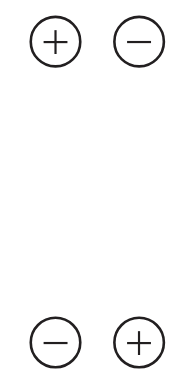
\includegraphics[width=0.3\textwidth]{uni1}
        \caption[]{\label{uni1}}
    \end{subfigure}
    \hfill
    \begin{subfigure}[b]{0.4\textwidth}
        \centering
        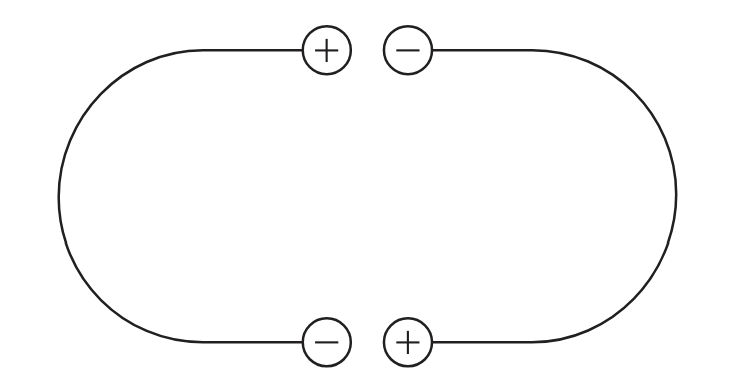
\includegraphics[width=\textwidth]{uni2}	
        \caption[]{\label{uni2}}
    \end{subfigure}
    
    \begin{subfigure}[b]{0.4\textwidth}
        \centering
        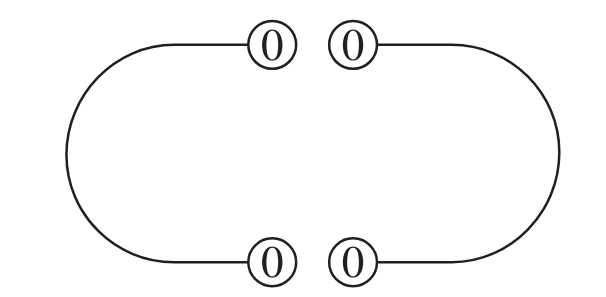
\includegraphics[width=\textwidth]{uni3}	
        \caption[]{\label{uni3}}
    \end{subfigure}
    
    \caption[]{\label{uni}}
\end{figure}

\example{A Variant to the Second Uniqueness Theorem.}
{Prove that the electric field is uniquely determined when \(\rho \) is given and either \(V \text { or } \pdv{V}{n} \) is specified on each boundary surface.}
{} 


\section{The Method of Images}

Suppose a point charge \(q\) is held a distance \(d\) above an infinite grounded conducting plane and we wish to find the potential in the region above the plane. From a mathematical standpoint, this is equivalent to solving the Poisson's equation in the region \(z > 0\), with \(\rho \) corresponds to a single point charge  \(q\) located at \((0,0,d )\), subject to the boundary conditions: 
\begin{enumerate}
    \item \(V = 0\) when \(z = 0\), and
    \item \(V \rightarrow 0\) for \(x^2 + y^2 + z^2 \gg d^2\).	
\end{enumerate}

By some clever insights, we see that for the potential created by a pair of opposite charge with \(q\) located at \((0,0,d)\) and \(-q\) located at \((0,0,-d)\) satisfy \(\rho \) in the region \(z > 0\)\footnote{We cannot place iamge charges in the volume \(V\) where we are calculating the potential, since for the first uniqueness theorem to stand, the charge density throughout the region has to be fixed as the given \(\rho \). Also the images charges must add up to the correct total in each region. (why?)} 

Since the electric field is just \(\vb{E} = -\grad{V} \), it is also uniquely determined and the force that the real charge experience can be easily calculated as \(\displaystyle \vb{F} = -\frac{1}{4\pi\epsilon_0} \frac{q^2}{(2d)^2} \vu{z}  \).

The potential energy of the system can be found by integrating the force from infinity to \(d\) which yields \(\displaystyle U = \int_{\infty}^{d} \frac{1}{4\pi\epsilon_0} \frac{q^2}{(2z)^2} dz = -\frac{1}{4\pi\epsilon_0} \frac{q^2}{4d}  \) which is only half of the energy of a pair of real charge \(q \text{ and }  -q\) separated by a distance \(2d\). 

This is because there is no electric field in the region \(z < 0\), or equivalently, the image charge can be moved for free, since there isn't any electric field to oppose. 

So in general the energy becomes \(U = q_{\text{real} } V \) and we only need to take into account the energy of the real charges. 

\example{Image Charges of a Conducting Spherical Shell.}
{A point charge \(q\) is situated a distance \(a\) from the center of a conducting shell\footnote{A conducting sphere works just as fine here as well. This is because for \(a > R\), the real charge density is zero inside the shell, so the internal field can be found by solving the Laplace's equation with \(\rho = 0\) and subject to the boundary condition of constant potential at the shell. By invoking the first uniqueness theorem, we see that the internal field equals to zero which resembles the case of a conductor is the only answer.} of radius \(R < a\)\footnote{The same can be done for \(R > a\) but we omit here for simplicity.}. Find the potential outside the spherical shell if it is  
\newline 
\begin{enumerate}[itemsep=10pt] 
    \item grounded\footnote{Grounded means \(V = 0 \) relative to infinity, since it is connected to the Earth by a wire, and Earth has infinite capacitance, if we consider the Earth and the sphere as one conductor, we get \(V = 0\) from \(Q = CV\).}, or
    \item held at potential \(V_0\), or
    \item isolated with net charge \(Q\).
\end{enumerate}~}
{\begin{enumerate}
    \item The problem is equivalent to solving the Laplace's equation for the region outside the sphere, subject to the boundary conditions: 
    
    \begin{enumerate}[itemsep=10pt] 
        \item \(V = 0\) on the surface of the sphere, and
        \item \(V \rightarrow 0\) for  \(x^2 + y^2 + z^2 \gg R\) .		
    \end{enumerate} 
    
    It so happens that the potential created by a point charge \(q' = -\frac{R}{a} q\) located at \(\frac{R^2}{a} \) from the center of the sphere (which always stay inside the sphere since \(R < a\)) together with the real charge satisfies both the boundary conditions and the charge density requirement. 
    
    Thus, by the first uniqueness theorem, the potential created by the two charges is our final and only answer.\newline 
    
    \item Now the boundary conditions are modified to be:
    
    \begin{enumerate}
        \item \(V = V_0\) on the surface of the sphere, and
        \item \(V \rightarrow 0\) for \(x^2 + y^2 + z^2 \gg R\).	 
    \end{enumerate}
    
    Then since from the first part we already know that the potential created by \(q \text{ and } q'\) is zero over the surface of the shell, we only need to add another image charge \(q''\) at the center of the shell (or over the surface of the shell) such that 
    
    \begin{equation}
        V_0 = \frac{1}{4\pi\epsilon_0} \frac{q''}{R}.
    \end{equation}
    
    We see that the potential created by \(q, q' \text{ and } q''\) satisfy both the charge density requirement as well as the boundary conditions. Therefore, we claim this as our answer. \newline
    
    \item In this part, the boundary conditions are identical to those in the previous part, except for the fact that \(V_0\) is not known but is determined by the total net charge \(Q\). 
    
    To determine the relation between them, we see that since the electric field outside the sphere which is created by the real point charge and the real induced charge can be regarded as being created by the real point charge and the image charge, the field outside the sphere created by the real induced charge is identical as the field outside the sphere created by the image charge. So we have
    
    \begin{equation}
        \oint _{S} \vb{E}_{\text{real, induced}}  \cdot d\vb{S} = \frac{q_{\text{real, induced}}}{\epsilon_0} = \oint _{S} \vb{E} _{\text{image}} \cdot d\vb{S} = \frac{q_{\text{image}}}{\epsilon_0} .
    \end{equation}
    
    Therefore we conclude that the image charge is equal to the induced charge. So if the total net charge of the shell is \(Q\), then  we have
    
    \begin{equation}
        Q = q' + q''.
    \end{equation}
    
    And the rest is identical to the previous part.
\end{enumerate}~} 


\section{Separation of Variables}

The method of separations of variables used for tackling the Laplace's equation is best illustrated with examples.

\subsection{Cartesian Coordinates}

In the Cartesian Coordinates, the Laplace's equation reads
    
\begin{equation}
    \frac{\partial V}{\partial x}  + \frac{\partial V}{\partial y}  + \frac{\partial V}{\partial z}  = 0. 
\end{equation}
            
We seek a solution in the form of 
    
\begin{equation}
    V(x,y) = X(x)Y(y)Z(z).
\end{equation}
    
Of course, the solution need not to be in this form. However, if we do find a solution, by any means, that satisfy the Laplace's equation and its boundary conditions, then by the first uniqueness theorem, we know that it must be the only answer. 
    
Substituting our proposed solution and separating the variables,
    
\begin{equation}
    \begin{aligned}
        Y \frac{d^2X}{dx^2} + X \frac{d^2Y}{dy^2} + Z \frac{d^2Z}{dz^2} &= 0 \\
        \frac{1}{X} \frac{d^2X}{dx^2} + \frac{1}{Y} \frac{d^2Y}{dy^2} + \frac{1}{Z} \frac{d^2Z}{dz^2} &= 0. 
    \end{aligned}
\end{equation}
    
Since we have an equation in the form of \(f(x) + g(y) + h(z) = 0\), the only way the this could possibly be true is that both  \(f,g \text{ and }  z\) must be constant or else I could say vary \(x\) while keeping \(y \text { and } z\) constant and the equality wouldn't hold. Thus, we have
    
\begin{equation}
    \frac{1}{X} \frac{d^2X}{dx^2} = C_1, ~~~\frac{1}{Y} \frac{d^2Y}{dy^2} = C_2 ~~~ \text{ and } ~~~ \frac{1}{Z} \frac{d^2Z}{dz^2} = C_3, ~~~ \text{ with }  C_1 + C_2 + C_3 = 0.
\end{equation}

\example{Separation of Variables in Cartesian Coordinates.}
{Find the potential \(V(x,y)\) bounded by the metal sheets fixed at potential \(V_0 (y)\) and infinity as shown in \cref{lap1}.}
{By symmetry, it is obvious that \(V\) is independent of \(z\), and the boundary conditions are
            
\begin{enumerate}[itemsep=10pt] 
    \item \(V = 0\) when \(y = 0 \text { and }  y = a\),
    \item \(V = V_0(y)\) when \(x = 0\), and
    \item \(V \rightarrow  0\) as \(x \rightarrow  \infty\).
\end{enumerate}

With the results derived, we have

\begin{equation}
    \frac{d^2X}{dx^2} = k^2X ~~~ \text{ and } ~~~ \frac{d^2Y}{dy^2} = -k^2Y
\end{equation}

where we rewrite the constant \(C_1 \text{ as } k^2\) since \(C_1\) should be positive and  \(C_2\) should be negative, such that \(V(x)\) will admit an exponential decaying function where \(V(x) \rightarrow 0\) as \(x \rightarrow \infty\) and \(V(y)\) will admit a sinusoidal function so that \(V(y)\) will vanish at \(y = 0\) and \(y = a\).            

which gives the solutions

\begin{equation}
    V(x,y) = (A e^{kx} + B e^{-kx} )(C\sin ky+D\cos ky) .
\end{equation}

Applying the boundary conditions 1 and 3 will left us with 

\begin{equation}
    V(x,y) = C e^{-kx} \sin ky, ~~~ \text{ where } k = \frac{n\pi }{a}. 
\end{equation}

Since the Laplace's equation is linear, the general solution is the linear combination of all solutions each with different \(n\), so we have 

\begin{equation}
    V(x,y) = \sum_{n=1}^{\infty} C_{n} \sin \frac{n\pi y}{a} e^{-\frac{n\pi x}{a}} .
\end{equation}

To satisfy the second boundary condition

\begin{equation}
    V(0,y) = \sum_{n=1}^{\infty} C_{n} \sin \frac{n\pi y}{a} = V_0(y) ,
\end{equation}

we have to rely on the Fourier's trick, where we multiply both sides by \(\sin \frac{m\pi y}{a} \) and integrate from \(0 \text { to } a\)

\begin{equation}
    \sum_{n=1}^{\infty} C_{n} \int_{0}^{a} \sin \frac{n\pi y}{a} \sin \frac{m\pi y}{a} dy = \int_{0}^{a} V_0(y) \sin \frac{m\pi y}{a} dy.			 
\end{equation}

Since 

\begin{equation}
    \int_{0}^{a} \sin \frac{n\pi y}{a} \sin \frac{m\pi y}{a} dy = \begin{cases}
        0 & \text{if } n \neq m, \\[10pt]
        \displaystyle \frac{a}{2} & \text{if } n = m.
        \end{cases}
\end{equation}

Thus 

\begin{equation}
    C_{n}  = \frac{2}{a} \int_{0}^{a} V_0(y) \sin \frac{n\pi y}{a} dy.  
\end{equation}

If \(V_0(y) = V_0\), then 

\begin{equation}
    \begin{aligned}
        C_{n} &= \frac{2v_0}{a} \int_{0}^{a} \sin \frac{n\pi y}{a} dy = \frac{2V_0}{n\pi } (1 - \cos n\pi )  \\ 
        &= \begin{cases}
            ~ 0 &\text { if } n  \text{ is even}, \\
            \frac{4V_0}{n\pi } &\text { if } n \text{ is odd} .
        \end{cases} 
    \end{aligned}
\end{equation}

Thus

\begin{equation}
    V(x,y) = \frac{4V_0}{\pi } \sum_{\text{odd n}}^{} \frac{1}{n} \sin \frac{n\pi y}{a}  e^{\frac{-n\pi x}{a}}. 
\end{equation}

Incidentally, the result can be further simplified by writing \(\displaystyle \sin \frac{in\pi y}{a} \text{ as } \mathfrak{Re} ((-i)e^{\frac{n\pi y}{a} } )  \), then \(\displaystyle V(x,y) = \frac{4V_0 }{\pi } I\), where

\begin{equation}
    I = \mathfrak{Re} \left(-i\sum_{\text{odd n}}^{} \frac{1}{n} \left(e^{-\frac{\pi (x-iy)}{a} }\right)^{n}\right) 
\end{equation}

Letting \(\displaystyle \mathcal{Z} = e^{-\frac{\pi (x-iy)}{a} }  \), we have

\begin{equation}
    \begin{aligned}
        \sum_{\text{odd n}}^{} \frac{\mathcal{Z} ^{n} }{n} &= \sum_{j=0}^{\infty} \frac{\mathcal{Z} ^{(2j+1)} }{2j+1} = \int_{0}^{\mathcal{Z} } \left(\sum_{j=0}^{\infty} u^{2j} \right)du = \int_{0}^{\mathcal{Z} } \frac{du}{1-u^2} \\
        &= \frac{1}{2} \ln (\frac{1+\mathcal{Z} }{1-\mathcal{Z} } ) = \frac{1}{2}  \ln (R e^{i\theta } ) = \frac{1}{2} (\ln R + i\theta )
    \end{aligned}
\end{equation}

where we have defined \(\displaystyle R e^{i\theta } \text{ as } \frac{1+\mathcal{Z} }{1-\mathcal{Z} } \). So \(\displaystyle I =  \mathfrak{Re}  ((-i)\frac{1}{2} (\ln R + i\theta )) = \frac{\theta }{2}  \). Since 
\begin{equation}
    \begin{aligned}
        &\frac{1+\mathcal{Z}}{1-\mathcal{Z}}=\frac{1+e^{-\pi(x-i y) / a}}{1-e^{-\pi(x-i y) / a}}=\frac{\left(1+e^{-\pi(x-i y) / a}\right)\left(1-e^{-\pi(x+i y) / a}\right)}{\left(1-e^{-\pi(x-i y) / a}\right)\left(1-e^{-\pi(x+i y) / a}\right)} \\
        & =\frac{1+e^{-\pi x / a}\left(e^{i \pi y / a}-e^{-i \pi y / a}\right)-e^{-2 \pi x / a}}{\left(1-e^{-\pi(x-i y) / a}\right)\left(1-e^{-\pi(x+i y) / a}\right)}=\frac{1+2 i e^{-\pi x / a} \sin (\pi y / a)-e^{-2 \pi x / a}}{\left(1-e^{-\pi(x-i y) / a}\right)\left(1-e^{-\pi(x+i y) / a}\right)}
    \end{aligned}
\end{equation}

for which the denominator is real, so

\begin{equation}
    \tan \theta=\frac{2 e^{-\pi x / a} \sin (\pi y / a)}{1-e^{-2 \pi x / a}}=\frac{2 \sin (\pi y / a)}{e^{\pi x / a}-e^{-\pi x / a}}=\frac{\sin (\pi y / a)}{\sinh (\pi x / a)}. 
\end{equation}


Therefore 
\begin{equation}
    I=\frac{1}{2} \tan ^{-1}\left(\frac{\sin (\pi y / a)}{\sinh (\pi x / a)}\right) \implies  V(x, y)=\frac{2 V_0}{\pi} \tan ^{-1}\left(\frac{\sin (\pi y / a)}{\sinh (\pi x / a)}\right) .
\end{equation}}

\onefig{lap1}{scale=0.3} 

\subsection{Spherical Coordinates}

Asuuming that the potential \(V\) is independent of \(\phi \), the Laplace's equation reads 

\begin{equation}
    \pdv{r} (r^2 \pdv{V}{r} ) + \frac{1}{\sin \theta } \pdv{\theta } (\sin \theta \pdv{V}{\theta } ) = 0.
\end{equation}

Substituting \(V(r,\theta ) = R(r)\Theta (\theta )\) and separating the variables, we have 

\begin{equation}
    \frac{1}{R} \frac{d}{dr} (r^2 \frac{dR}{dr} ) = l(l+1) ~~~ \text{ and } ~~~ \frac{1}{\Theta \sin \theta } \frac{d}{d\theta} (\sin \theta \frac{d\Theta}{d\theta} ) = -l(l+1)	
\end{equation}

where we have written the separation constant as \(l(l+1)\) where \(l\) is an positive integer, or else the solution would not be physical on the \(z\) axis as the series solution to the angular differential equation would not converge for \(\theta = 0 \text { or }  \pi \) explained \href{https://jfoadi.me.uk/documents/lecture_mathphys2_08.pdf}{here}.

For the radial ordinary differential equation, the general solution has the form

\begin{equation}
    R(r) = Ar^{l} + \frac{B}{r^{l+1} } .
\end{equation}

While for the angular ordinary differential equation, the general solutions are Legendre polynomials in the variable \(\cos \theta \), where is given by the Rodrigues formula

\begin{equation}
    P_{l}(x) = \frac{1}{2^{l} l!} \left(\frac{d}{dx} \right)^{l} (x^2 - 1)^{l} . 
\end{equation}

The first few Legendre Polynomials are \(P_0(x) = 1, ~P_1(x) = x \text{ and } P_2(x) = \frac{3x^2 - 1}{2} \). Also, with the factor \(\frac{1}{2^{l} l!} \) introduced, we have \(P_{l} (1) = 1\).  

However since the angular differential equation is second order, it should possess two independent solutions for every value of \(l\). It turns out that the other solution blow up at the \(z\) axis anyways and is eliminated by initial or boundary conditions such that the coefficient introduced due to the linearity of the differential equation becomes zero.

From the linearity of the Laplace's equation, the general solution is

\begin{equation}
    V(r,\theta ) = \sum_{l=0}^{\infty} (A_{l} r^{l} + \frac{B_{l} }{r^{l+1} } )P_{l} (\cos \theta). \label{sphlap1} 
\end{equation}

\example{Separation of Variables in Spherical Coordinates (1).}
{Find the potential in all space if \(V_0(\theta )\) is specified on a spherical shell of radius \(R\).}
{For the region inside the shell, we immediately see that \(B_{l} = 0\) otherwise the potential would blow up at the origin. Also, we require that 

\begin{equation}
    V(R,\theta ) = \sum_{l=0}^{\infty} A_{l} R^{l} P_{l} (\cos \theta ) = V_{0} (\theta )
\end{equation}

We again use the Fourier's trick, but this time we multiply by \(P_{l'} (\cos \theta )\) and use the fact that 

\begin{equation}
    \begin{aligned}
        \int_{-1}^{1} P_{l} (x) P_{l'} (x) dx &= \int_{0}^{\pi } P_{l} (\cos \theta ) P_{l'} (\cos \theta ) \sin \theta d\theta \\ &= \begin{cases}
            ~~0 & \text{if } l' \neq l \\[10pt]
            \displaystyle \frac{2}{2l+1} & \text{if } l' = l.
            \end{cases}
    \end{aligned}
\end{equation}

Thus by similar means as the previous example, we get

\begin{equation}
    A_{l} = \frac{2l+1}{2R^{l} } \int_{0}^{\pi } V_{0} (\theta ) P_{l} (\cos \theta ) \sin \theta d\theta.
\end{equation}

The integrals can be difficult to evaluate and in practice it is often easier to solve for \(A_{l} \) by observation. For example, if \(\displaystyle V_0(\theta ) = k\sin ^2\left(\frac{\theta }{2} \right)\), then we can rewrite this as

\begin{equation}
    V_0(\theta ) = \frac{k}{2} (1-\cos \theta ) = \frac{k}{2} (P_0(\cos \theta ) - P_1(\cos \theta )).
\end{equation}

So we immediately read off from \cref{sphlap1} that \(\displaystyle A_0 = \frac{k}{2} \text{ and }  A_1 = -\frac{k}{2R} \) and

\begin{equation}
    V(r,\theta )  = \frac{k}{2} (1 - \frac{r}{R} \cos \theta ).
\end{equation}	

And if \(V_0(\theta) = k\cos (3 \theta)\), then we can rewrite this as

\begin{equation}
    V_0(\theta) = k(4\cos ^3 \theta - 3\cos \theta) = \frac{k}{5} (8P_3 (\cos \theta) - 3P_1(\cos \theta)).
\end{equation}

So we can find that \(\displaystyle A_1 = -\frac{3k}{5R} \text{ and } A_3 = \frac{8k}{5R^3} \) and 

\begin{equation}
    V(r,\theta) = \frac{kr\cos \theta}{5R} \left(4\left(\frac{r}{R}\right)^2(5\cos ^2 \theta-3)-3\right). 
\end{equation}} 


\example{Separation of Variables in Spherical Coordinates (2).}
{Find the potential in the region outside of an uncharged metal sphere of radius \(R\) placed in an otherwise unifrom electric field \(\vb{E} = E_0 \vu{z} \).}
{Since \(V\) does not goes to zero at infinity, we redefine the potential to be zero at the surface of the sphere (since it is an equipotential surface). Then the boundary conditions becomes
    
\begin{enumerate}[itemsep=10pt] 
    \item \(V = 0 \text { at } r = R\),
    \item \(V \rightarrow -E_0z = -E_0r\cos \theta \text { for } r \gg R\). 
\end{enumerate}

Applying the first boundary condition gives

\begin{equation}
    V(r,\theta ) = \sum_{l=0}^{\infty} A_{l} \left(r^{l}  - \frac{R^{2l+1} }{r^{l+1} } \right) P_{l} (\cos \theta ). 			
\end{equation}

And the second boundary condition requires that 

\begin{equation}
    \sum_{l=0}^{\infty} A_{l} r^{l} P_{l} (\cos \theta ) = -E_0 r\cos \theta .  
\end{equation}

Thus, we read off \(A_{l} = 0\) except for \(A_1 = -E_0 \) and the potential is 

\begin{equation}
    V(r,\theta ) = -E_0 \left(r-\frac{R^3}{r^2} \right) \cos \theta 
\end{equation}

where the first term is due to the external field and the second term is contributed by the induced charge.

The induced charge density can be calculated by 

\begin{equation}
    \sigma (\theta ) = -\epsilon_0 \eval{\pdv{V}{r} }_{r=R}^{} = 3 \epsilon_0	E_0 \cos \theta  
\end{equation}} 

\example{Separation of Variables in Spherical Coordinates (3).}
{A specified charge density \(\sigma_0(\theta)\) is glued over the surface of a spherical shell of radius \(R\). Find the resulting potential inside and outside the sphere without using \cref{potential}.}
{We start with 

\begin{equation}
     V(r, \theta) =
    \begin{cases}
    \displaystyle \sum_{l=0}^{\infty} A_{l}r^{l}P_{l}(\cos \theta )    & \text{for } r \leq R, \\[10pt]
    \displaystyle \sum_{l=0}^{\infty} \frac{B_{l} }{r^{l+1} } P_{l}(\cos \theta ) & \text{for } r \geq R.
    \end{cases}  
\end{equation}

The boundary conditions are that the two potentials must be the same at \(r = R\) and the difference in nomral derivatives is due to the presence of the surface charge. So

\begin{equation}
    \sum_{l=0}^{\infty} A_{l}R^{l}P_{l}(\cos \theta ) = \sum_{l=0}^{\infty} \frac{B_{l} }{R^{l+1} } P_{l}(\cos \theta ) ~\text { and }~ \eval{\left( \frac{\partial V_{\text{out} } }{\partial r} - \frac{\partial V_{\text{in} } }{\partial r}   \right)}_{r=R}^{} = -\frac{\sigma _{0}(\theta ) }{\epsilon _{0} }.         
\end{equation}

They combined to give 

\begin{equation}
    A_{l} = \frac{1}{2\epsilon _{0}R^{l-1}  } \int_{0}^{\pi } \sigma _{0}(\theta ) P_{l}(\cos \theta ) \sin \theta d \theta ~\text { and }~ B_{l} = A_{l}R^{2l+1}.       
\end{equation}

For instance, if \(\sigma _{0} = k\cos \theta  = kP_1 (\cos \theta )\), then \(\displaystyle A_1 = \frac{k}{3\epsilon _{0} }\) which impiles 

\begin{equation}
      V(r, \theta) =
    \begin{cases}
    \displaystyle \frac{k r \cos\theta}{3 \epsilon_0}, & \text{for } r \leq R \\[10pt]
    \displaystyle \frac{k R^3 \cos\theta}{3 \epsilon_0 r^2} & \text{for } r \geq R.
    \end{cases}  
\end{equation}

In particular, we found from the previous example that the induced charge of a metal sphere under an otherwise uniform electric field \(\vb{E} = E_0 \vu{z} \) is \(\sigma _{0}(\theta ) = 3 \epsilon _{0}E_0   \). Subsituting \(k = 3 \epsilon _{0}E_0  \), we see that the potential inside is \(V(r,\theta ) = E_0 r \cos \theta = E_0 z\) and the field is \(- E_0 \vu{z} \) which cancels out the external field \(E_0 \vu{z} \), as it should.      
} 


The success of the method of separation of variables hinges on two extraordinary properties of the separable solutions, namely the completeness and orthogonality. In linear algebra terms, the set of functions is an orthonormal basis of the set of all real functions.

A set of functions \(f_{n} (y)\) is said to be complete if any other function \(f(y)\) can be expressed as a linear combination of them, \textit{i.e.,} 

\begin{equation}
    f(y) = \sum_{n=1}^{\infty} C_{n} f_{n} (y). 
\end{equation}

For example, the functions \(\sin \frac{n\pi y}{a}\), where \(n\) are positive integers are complete over the interval \(0~\le~y\le~a\) as guaranteed by Dirichlet's theorem. Also, any \(n^{\text{th }} \)  order polynomials can be expressed as the linear combination of the first \(n+1\) Legendre's polynomials, as the set of functions \(P_{l} (x)\) is complete for polynomials.

Orthogonality, on the other hand, means that the integral of the product of any two distinct members of the set is zero, \textit{i.e.,}  
\begin{equation}
    \int_{0}^{a} f_{n} (y) f_{n'} (y) dy = 0 \text { for }  n' \neq n. 
\end{equation}

It is this property that allows us to perform the Fourier's trick.


\chapter{Electric Field in Matter}

\section{Multipole Expansion and Dipole moment}

Referring to \cref{multipoleexpansion}, suppose we are trying to find the potential (or equivalently, electric field) of a point \(P\) in space far away from the source charges. We then have 

\onefig{multipoleexpansion}{scale=0.3} 

\begin{equation} \label{1drj} 
    \begin{aligned} 
    \frac{1}{\rcurs } &= \frac{1}{ r \sqrt{1 - 2\cos \alpha \left( \frac{r'}{r}  \right) + \left( \frac{r'}{r}  \right)^2}} \equiv \frac{1}{r} (1 + \epsilon )^{-\frac{1}{2} } = \frac{1}{r} \left( 1 - \frac{1}{2}\epsilon  + \frac{3}{8} \epsilon ^2 + \frac{5}{16} \epsilon ^3 + \cdots  \right) \\
    &=\frac{1}{r} \left( 1 + \cos \alpha \left( \frac{r'}{r}  \right) + \left( \frac{3\cos ^2\alpha -1}{2} \right) \left( \frac{r'}{r}  \right)^2 -\frac{5}{16} \left( \frac{5\cos ^3 \alpha - 3\cos \alpha }{2} \right) \left( \frac{r'}{r} \right)^3 + \cdots \right) \\
    &= \frac{1}{r} \sum_{n=0}^{\infty} \left( \frac{r'}{r}  \right)^{n} P_{n}(\cos \alpha ),  
    \end{aligned} 
\end{equation}

where \(\alpha \) is the angle between \(\vb{r} \text { and } \vb{r} '\) and \(P_{n}\) is the \(n^{\text{th }} \) Legendre polynomials.    

Substituting back into \cref{comb}, we have 

\begin{equation}
    \begin{aligned} 
    V(\vb{r} ) &= \frac{1}{4\pi \epsilon _0} \sum_{n=0}^{\infty} \frac{1}{r^{n+1} } \int r'^{n} P_{n}(\cos \alpha )\rho (\vb{r} ')d\tau ' \\
    &= \frac{1}{4\pi \epsilon_0} \left( \frac{1}{r} \int \rho (\vb{r} ')d\tau ' + \frac{1}{r^2}\int r'\cos \alpha \rho (\vb{r} ')d\tau ' + \cdots  \right) 
    \end{aligned} 
\end{equation}

The first term is the monopole contribution, telling that if we are sufficiently far away from the source, then we can treat the charge distribution as a point charge at the origin, which vanishes if the total charge is zero.

The second term is the dipole contribution, which can be written as 

\begin{equation}
    V_{\text{dip} } (\vb{r} ) = \frac{1}{4\pi \epsilon_0r^2} \left( \vu{r}  \cdot \int \vb{r} ' \rho (\vb{r} ')d\tau '  \right) = \frac{\vb{p} \cdot \vu{r} }{4\pi \epsilon _0 r^2 }.    
\end{equation}

Analagous to a point charge at the origin where its potential is exactly given by the first term of the multipole expansion, a perfect dipole whose potential is exactly given by the second term of the multipole expansion is when 

\begin{equation}
    \vb{p} = \lim_{\vb{d}  \to 0, q \to \infty} q\vb{d}  
\end{equation}

and is located at the origin. 

The terms in the multipole expansion generally depends on the choice of origin. however, if the total charge is zero, then the dipole term is independent of the choice of origin. This is also the reason why the dipole moment of two opposite charge with the same magnitude \(q\) is simply \(\vb{p} = q\vb{d} \), where \(\vb{d} \) is the displacement vector from the negative charge to the positive charge. 

Placing the dipole at the origin, orienting \(\vb{p} \) to point in the \(z\) direction and taking the negative gradient of the potential contributed by the dipole term, we get the electric field created by a dipole as

\begin{equation}
    \vb{E} _{\text{dip} } (r, \theta ) = \frac{p}{4\pi \epsilon _0 r^3 }(2\cos \theta \vu{r} + \sin \theta \vu{\boldsymbol{\theta } }). 
\end{equation}










\section{Polarization}

A material can be classified into either a conductor, where there are unlimited supply of free charges that can move around, or an insulator (or dielectric), where there are no free charges that can move around the material. 

Just as a conductor will response to an external electric field \(\vb{E} _{\text{ext} } \)  by moving the free charges around which creates an opposing electric field that cancels out with the external one, such that the electric field inside a conductor is zero, a dielectric material would also response to an electric field in a similar way, cancelling the external electric field partially. In fact, a conductor is merely an extreme case of a very bad insulator (\(\chi _{e} \to \infty\) ).

This is because the electric field will cause a lot of little electric dipoles to appear, for which the effect is measured by the polarization \(\vb{P} \) which is the dipole moment per unit volume. The two mechanisms causing the polarization are not important but are stated below.

The relation between \(\vb{P} \text { and } \vb{E} \) of a material is charizterized by its electric susceptibility 

\begin{equation}
    \vb{P} = \epsilon _{0} \chi _{e}\vb{E}_{\text{tot} }.
\end{equation}

An important point to note here is that \(\vb{E} _{\text{tot} } \) comprise of both the electric field which already exists before the polarization, as well as the electric field created by the induced bound charges due to polarization. 

\subsection{Ionization of Non-Polar Atoms}

As the force experienced by the positive nucleus and the negative electron cloud is in opposite direction, they will drift towards opposite direction until the attraction force between the nucleus and the electron cloud balance the the electric force exerted by the external electric field. The induced dipole moment of the atom \(\vb{p} \) is given in terms of the atomic polarizability \(\alpha \) as \(\vb{p} = \alpha \vb{E}_{ext}  \).

\example{Atomic Polarizability.}
{Calculate the atomic polarizability for an atom with radius \(\vb{a} \) and nucleus charge \(+q\).}
{Let \(d\) be the distance between the nucleus and the center of the electron cloud when the atomic reaches an equilibrium state. Balancing the forces on the nucleus (or the electron cloud), we have

\begin{equation}
    qE_{\text{ext} }  = q \frac{1}{4\pi \epsilon_0} \frac{qd}{a^3 }.
\end{equation}

The atomic polarizability is therefore 

\begin{equation}
    \alpha = \frac{p}{E_{ext} } =  \frac{qd}{E_{ext} } = 4\pi \epsilon _0 a^3 = 3\epsilon _0 V. 
\end{equation}
} 

\subsection{Alignment of Polar Molecules} \label{alignpolar} 

The force and the torque about its center expereinced by a molecule (which we model as an electric dipole) is 

\begin{equation}
    \vb{F} = q(\Delta \vb{E} ) = q (\grad{\vb{E} } \cdot \vb{d}) = (\vb{p}  \cdot \boldsymbol{\nabla }) \vb{E} ~\text { and }~ \vb{N} = \vb{p} \cross \vb{E}
\end{equation}

and the energy of a dipole is 

\begin{equation}
    U = q(V(\vb{r} + \vb{d} ) - V(\vb{r} )) = q\Delta V(\vb{r} ) = q\grad{V(\vb{r} )}\cdot \vb{d} = - \vb{p} \cdot \vb{E}. 
\end{equation}

So the molecules will align themselves towards the direction of the elctric field in order to achieve minimum energy. 

\section{The Electric Fields of Polarized Objects}

To calculate the electric field due to a polairized object, we notice tha the potential from \cref{potential} reads

\begin{equation}
    \begin{aligned} 
    V(\vb{r} ) &= \frac{1}{4\pi \epsilon_0} \int_{V}^{} \frac{\vb{P} (r')\cdot \hrcurs }{\rcurs ^2}d\tau ' = \frac{1}{4\pi \epsilon_0} \int_{V}^{} \vb{P} \cdot \boldsymbol{\nabla '}\left( \frac{1}{\rcurs }  \right) d\tau ' \\
    &= \frac{1}{4\pi \epsilon_0} \left( \int_{V}^{} \boldsymbol{\nabla '} \cdot \left( \frac{\vb{P} }{\rcurs }  \right) d\tau ' - \int_{V}^{} \frac{1}{\rcurs } (\boldsymbol{\nabla '} \cdot \vb{P}  ) d\tau ' \right) \\
    &= \frac{1}{4\pi \epsilon_0} \left( \oint_{S} \frac{1}{\rcurs }\vb{P} \cdot d\vb{S} '  - \int_{V}^{} \frac{1}{\rcurs } (\boldsymbol{\nabla '} \cdot \vb{P}  ) d\tau ' \right) \\
    &= \frac{1}{4\pi \epsilon_0} \left( \oint_{S} \frac{\sigma _{b} }{\rcurs } dS' + \int_{V}^{} \frac{\rho _{b} }{\rcurs } d\tau ' \right),
    \end{aligned} 
\end{equation}

where \(\sigma _{b} = \vb{P} \cdot \vu{n} \text { and } \rho _{b} = - \div{\vb{P} } \) are the surface and volume charge density result from the polarization respectively.

The introduction of surface and volume bound charges is not merely a bookeeping tool, but are in fact visualizable. 

For surface bound charge, we imagine a long string of dipoles, where the positive head of one cancels the negative tail of its neighbor, so what left is the plus hand and the minus tail.

Since \(qd = PAd\) is the diopole moment of one individual dipole, we have the surface charge density as \(\sigma _{b} = \frac{q}{A} = P\), where the dot product with the normal unit vector is introduced to taken into account if the end surface is not perpendicular to the polarization, then the area would be larger by a factor of \(\cos \theta \), where \(\theta \) is the angle between the polarizatoin and the unit normal vector.

For volume bound charge, we imagine some volume with non-zero divergence of polarization. Then by conservation of charge we have the amount positive charges reside on the surface of the volume (which in this case are effectively surface charges) is equal to amount of the negative charge inside the volume, so

\begin{equation}
    \int_{V}^{} \rho _{b} d\tau = - \oint_{S} \vb{P} \cdot d\vb{S} = - \int_{V}^{} (\div{\vb{P} } )d\tau . 
\end{equation}

Therefore, we can first calculate these induced bound charge (which are charges result from polarization) then calulcate the electric field via normal means.

\example{Uniformly Polarized Sphere (1).}
{Find the electric field produce by a uniformly polarized sphere of radius \(R\) and polarization \(\vb{P} \).}
{The surface and volume charge density are

\begin{equation}
    \sigma _{b} = \vb{P} \cdot \vu{n} = P\cos \theta  ~\text { and }~ \rho _{b} = - \div{\vb{P} } = 0.  
\end{equation}

But the problem of finding the potential of a surface charge density \(\sigma _{0} (\theta ) = k\cos \theta  \) glued on a sphere has alrady been solved in an example in the previous chapter. The result therefore is

\begin{equation}
 V(r, \theta) =
    \begin{cases}
    \displaystyle \frac{P r \cos\theta}{3 \epsilon_0} & \text{for } r \leq R, \\[10pt]
    \displaystyle \frac{P R^3 \cos\theta}{3 \epsilon_0 r^2} & \text{for } r \geq R.
    \end{cases}  
\end{equation}

The electric field inside the sphere is 

\begin{equation}
    \vb{E} = -\grad{V} = - \frac{\vb{P} }{3\epsilon _{0} }\vu{z} = - \frac{\vb{P} }{3 \epsilon _{0} } \text{ for } r \le R
\end{equation}

while the potential outside the sphere is 

\begin{equation}
    V = \frac{1}{4\pi \epsilon_0} \frac{\vb{p} \cdot \vu{r} }{r^2} \text{ for } r \ge R, 
\end{equation}

which is indentical to that of a perfect dipole at the origin with dipole moment \(\vb{p} = \frac{4}{3}\pi R^3 \vb{P}  \) which is the total dipole moment of the sphere. 
} 

\example{Uniformly Polarized Sphere (2).}
{Analyze the same uniformly polarized sphere in the previous example by considering two overlapping spheres of charges \(+q\text { and } -q\).}
{The total electric field inside the overlapping region is the sum of the electric field of the individual spheres, which can be shown to be equals to

\begin{equation}
    \vb{E} = -\frac{1}{4\pi \epsilon_0} \frac{q\vb{d} }{R^3 } = -\frac{\vb{P} }{3\epsilon _{0} } 
\end{equation}

For the region outside the spheres, it is as though all the cahrges on each sphere were concentrated at the respective centers. We have then a dipole with potential 

\begin{equation}
    V(\vb{r} ) = \frac{1}{4\pi \epsilon_0} \frac{\vb{p} \cdot \vu{r} }{r^2}. 
\end{equation}
} 

\section{Microscopic and Macroscopic Fields}

When we say the electric field inside a point in matter, we do not mean the acutual microscopic electric field at that point, as the microscopic fields are actually highly non-uniform. What we meant is always the average electric field over a small region which is large enough to smooth over the uninteresting microscopic fluctuations and yet small enough to not wash out any significant large-scale variations in the field. 

Suppose we would like to find \(\vb{E} (\vb{r} )\) by averaging the true microscopic field over a small sphere about \(\vb{r} \) 

\section{Modified Gauss's Law}

While Gauss's law work copmletely fine inside matter, it would be more convenient to separate the electric field created by the induced bound charges \(\rho _{b} = -\div{\vb{P} } \) which are charges araised from polarization and the elctric field created by the free charges \(\rho _{f} \) which are charges not arised from polarization.

Introducing the electric displacement 

\begin{equation}
    \vb{D} = \epsilon _{0}\vb{E} + \vb{P} = \epsilon \vb{E}  ,  
\end{equation}

where \(\epsilon = \epsilon _{0}(1 + \chi _{e} ) = \epsilon _{0}\epsilon _{r}   \). 

So the ordinary Gauss's law can be rewritten to the modified Gauss's law

\begin{equation}
    \div{\vb{D} } = \rho _{f}. 
\end{equation}

The electric displacemnet is a useful quantity as when we put free charge in place, the only thing we know would be \(\vb{D} \) from the modified Gauss's law (instead of \(\vb{E} \) since we do not know \(\vb{P} \)).

However, we shall not assume that the relation between \(\vb{D} \text { and } \rho _{f} \) is the same as \(\vb{E} \text { and } \rho \). Although the divergence are analogous, the curl of \(\vb{E} \) is always zero while the curl of \(\vb{D} \) is \(\curl{\vb{D} } = \curl{\vb{P} } = \epsilon _{0}  \curl{\chi _{e} \vb{E} }  \) is not necessarily zero

But for the case of homogenous medium, where the electric susceptibiliy \(\chi _{e} \) does not vary with position, so \(\chi _{e} \) can be taken out of the curl and we can safely regard \(\rho _{f} \) as the source of \(\vb{D} \) just as how \(\rho \) serves as the source of \(\vb{E} \).        

For ionic crystal such as sodium chloride, where the polarization and thus electrical displacement is ill-defined as the direction of a dipole moment of two oppositely charged ions depends on how you pair them up. But it does not matter. At the end of the day everyone agrees that the charge density and the electric field is zero.  

\example{Separation of Variables in Spherical Coordinates (4).}
{A sphere of homogeneous linear dielectric material of relative permittivity \(\epsilon _{r} \) is placed in an otherwise uniform electric field \(\vb{E} _{0} \). Find the electric field inside the sphere.}
{Defining the zero potential at the center of the sphere, we need to solve the Laplace's equation subject to the boundary conditions

\begin{enumerate}[itemsep=10pt] 
    \item $V_{\text{in}} = V_{\text{out}}$ at $r = R$,
    \item $\displaystyle \epsilon \frac{\partial V_{\text{in}}}{\partial r} = \epsilon_0 \frac{\partial V_{\text{out}}}{\partial r}$ at $r = R$, and
    \item $V_{\text{out}} \to -E_0 z = -E_0 r \cos\theta$ for $r \gg R$.
\end{enumerate}

Inside the sphere, we have

\begin{equation}
    V_{\text{in} }(r, \theta ) = \sum_{l=0}^{\infty} A_{l} r^{l}P_{l}(\cos \theta ),
\end{equation}

where \(B_{l} = 0\) for all \(l\) to avoid singularities at the origin. 

Outside the sphere, we have

\begin{equation}
    V_{\text{out} }(r,\theta ) = -E_0 r\cos \theta + \sum_{l=0}^{\infty}\frac{B_{l} }{r^{l+1} }P_{l}(\cos \theta ),   
\end{equation}

where \(A_{l} = 0 \) for all \(l\) except \(A_1 = -E_0 \) to satisfy the third boundary condition.

Solving for \(A_{l} \text { and } B_{l}  \) with the first and second boundary conditions, we get 

\begin{equation}
    \begin{cases}
        A_l = B_l = 0 & \text{for } l \neq 1, \\[10pt]
        A_1 = \displaystyle -\frac{3}{\epsilon_r + 2} E_0, \\[10pt]
        B_1 = \displaystyle \frac{\epsilon_r - 1}{\epsilon_r + 2} R^3 E_0.
        \end{cases}   
\end{equation}

The potential and electric field inside the sphere are thus

\begin{equation}
    \begin{cases}
        V_\text{in}(r, \theta) = \displaystyle -\frac{3 E_0}{\epsilon_r + 2} z, \\[10pt]
        \mathbf{E} = \displaystyle \frac{3}{\epsilon_r + 2} \mathbf{E}_0.
        \end{cases}
\end{equation}

Note that \(\vb{E} = 0\) when \(\epsilon _{r} \to \infty\) as it should in the case of a conductor, and \(\vb{E} = \vb{E} _{0} \) when \(\epsilon _{r} = 1 \) as it should in the case of vaccum.    
} 

\example{Image Charge of an Infinite Dielectric Plane.}
{Suppose the entire region below the plane \(z=0\) is filled with uniform linear dielectric material of susceptibility \(\chi _{e} \). Calculate the force on a point charge \(q\) situated a distance \(d\) above the origin.}
{First of all, the volume bound charge is zero, since

\begin{equation}
    \rho _{b} = - \div{\vb{P} } = - \div{\left( \vb{D} - \epsilon _{0}\vb{E} \right)} = - \div{\left( \left(1- \frac{\epsilon _{0} }{\epsilon } \right) \vb{D} \right)} = - \left( 1- \frac{1}{\epsilon _{r} }  \right) \rho _{f} = 0.   
\end{equation}

The surface bound charge, on the other hand, is

\begin{equation}
    \sigma _{b} = \vb{P} \cdot \vu{n} = \epsilon _{0} \chi _{e}E_{z},    
\end{equation}

where \(E_{z} \) is the \(z-\)component of the total electric field just inside the dielectric at \(z=0\). This field is due in part to \(q\) and in part to the bound charge itself, so 

\begin{equation}
    E_{z} = - \left( \frac{1}{4\pi \epsilon_0} \frac{qd}{(r^2+d^2)^{\frac{3}{2} } } + \frac{\sigma _{b} }{2\epsilon _{0} }  \right).
\end{equation}

Solving for \(\sigma _{b} \), 

\begin{equation}
    \sigma _{b} = - \frac{1}{2\pi }\left( \frac{\chi _{e} }{\chi _{e}+2 }  \right)\frac{qd}{(r^2+d^2)^{\frac{3}{2} } }.   
\end{equation}

The electric field can be calculated by direction integration from \cref{comb} having known \(\sigma _{b} \). Alternatively, we note that we can place an image charge at \((0,0,-d)\) with charge \(\displaystyle q_{b} = -\frac{\chi _{e} }{\chi _{e}+2 } q \) we have the correct potential in the region \(z > 0\). For region \(z < 0\), we can place the same point charge at \((0,0,d)\).

Therefore the force is 

\begin{equation}
    \vb{F} = - \frac{1}{4\pi \epsilon_0} \left( \frac{\chi _{e} }{\chi _{e}+2 }  \right) \frac{q^2}{4d^2}\vu{z} . 
\end{equation}
} 

\section{Energy in Dielectric Systems}

The general formula for the electric energy \(\displaystyle U = \frac{\epsilon _{0} }{2} \int E^2d\tau  \) is generally not used in dielectric system. This is because this is the work done needed if we assemble the system by bringing in all the charges (free and bound), one by one, with tweezers to its proper final location. 

This energy, however, just not include the work done need stretch and rotate the atoms or molecules, which can be modelled as a spring's energy \(\displaystyle \frac{1}{2}kx^2 \),\footnote{For example, the restoring force of ionizing an atom is proportional to the relative displacement of the nucleus and the center of the electron cloud. So the energy is proportional to the displacemnet squared} which, although is electrical in nature, is not accounted in the macroscopic field \(\vb{E} \). 

The energy we are interested in, is the work done required to introduce all the free charges one by one to achieve the final configuation, while the energy due to bound charges are subtly accounted as the when we bring in an infinitesimal free charge, it also has to overcome the electric field created by the bound charge. Specifically, the infinitesimal work done required is 

\begin{equation}
    \begin{aligned} 
    \Delta W &= \int (\Delta \rho _{f} ) V d\tau = \int \left( \div{(\Delta \vb{D} )}  \right) Vd\tau = \int \div{\left( (\Delta \vb{D} ) V\right)} d\tau + \int \left( \Delta \vb{D}  \right) \cdot \vb{E} d\tau \\
    &= \oint_{S} \left( (\Delta \vb{D} )V \right) \cdot d\vb{S} + \int \left( \Delta \vb{D}  \right) \cdot \vb{E} d\tau = \int \epsilon (\Delta \vb{E} )\cdot \vb{E} d\tau = \frac{1}{2}\int \vb{D} \cdot \vb{E} d\tau . 
    \end{aligned} 
\end{equation}

where the potential is constant since we are bringing an infinitesimal charge into the system, so the potential should be the pre-exisiting potential.

So the total energy of a dielectric system is 

\begin{equation}
    U = \frac{1}{2} \int \vb{D} \cdot \vb{E} d\tau  .
\end{equation}

\example{Energy in a Dielcetric System.}
{A sphere of radius \(R\) is filled with material of dielectric constant \(\epsilon _{r} \) and uniform embedded free charge \(\rho _{f} \). Find the energy of this configuration.}
{From Gauss's law, we have

\begin{equation}
    \mathbf{D}(\mathbf{r}) =
    \begin{cases}
    \displaystyle \frac{\rho_f}{3} \mathbf{r} & \text{for } r < R, \\[10pt]
    \displaystyle \frac{\rho_f R^3 }{3r^2} \hat{\mathbf{r}} & \text{for } r > R,
    \end{cases}
    \implies 
    \mathbf{E}(\mathbf{r}) =
    \begin{cases}
    \displaystyle \frac{\rho_f}{3 \epsilon_0 \epsilon_r} \mathbf{r} & \text{for } r < R, \\[10pt]
    \displaystyle \frac{\rho_f R^3}{3 \epsilon_0 r^2} \hat{\mathbf{r}} & \text{for } r > R.
    \end{cases}
\end{equation}

So the pure electrostatic energy is 

\begin{equation}
    U_{\text{elec} }  = \frac{\epsilon _{0} }{2}  \int E^2d\tau = \frac{2\pi }{9\epsilon_0 }\rho _{f}^2R^{5}\left( \frac{1}{5\epsilon _{r}^2 }-1  \right)   
\end{equation}

while the total energy is 

\begin{equation}
    U_{\text{tot} }  = \frac{1}{2} \int \vb{D} \cdot \vb{E} d\tau =  \frac{2\pi }{9\epsilon_0 }\rho _{f}^2R^{5}\left( \frac{1}{5\epsilon _{r} }-1  \right)
\end{equation}

Of course, we can also do it in the most fundamental way, which is by assebling the system from scratch.

The electric field when a sphere of radius \(r'\) is already filled with uniform free charge is 

\begin{equation}
    \vb{E}  =
    \begin{cases}
        \displaystyle\frac{\rho_f}{3 \epsilon_0 \epsilon_r} \mathbf{r}, & \text{for } r < r', \\[10pt]
        \displaystyle\frac{\rho_f}{3 \epsilon_0 \epsilon_r} \frac{r'^3}{r^2} \hat{\mathbf{r}} & \text{for } r' < r < R, \\[10pt]
        \displaystyle\frac{\rho_f}{3 \epsilon_0} \frac{r'^3}{r^2} \hat{\mathbf{r}} & \text{for } r > R.
    \end{cases}
\end{equation}

So the infinitesimal work done to bring in an infinetisimal charge \(dq = \rho _{f} 4\pi r'^2dr'\) is 

\begin{equation}
    dW = - dq\int_{\infty}^{r'}\vb{E} \cdot d\vb{r} = \rho _{f}4\pi r'^2 \left(\frac{\rho _{f}r'^3  }{3 \epsilon_0 }\right)\left( \frac{1}{R} + \frac{1}{\epsilon _{r} }\left( \frac{1}{r'}-\frac{1}{R}   \right)   \right)dr'    
\end{equation}

Integrating, we get the same answer as the total energy.


We can also verify that the difference in them is indeed the work done requried to strech and rotate the particles. 

Let the restoring force be \(-k\vb{d} \), then we have \(q\vb{E} = k\vb{d} \) at equilibrium, where \(\vb{E} = \frac{\rho _{f} }{3\epsilon_0 \epsilon _{r} }\vb{r}  \), so the spring constant is 

\begin{equation}
    \begin{aligned} 
    k &= q\frac{\vb{E} }{\vb{d} } = \frac{q\rho _{f} r}{3\epsilon_0 \epsilon _{r} d} = \frac{p\rho _{f} r}{3\epsilon_0 \epsilon _{r} d^2} = \frac{P\rho _{f} r}{3\epsilon_0 \epsilon _{r} d^2} d\tau \\
    &= \frac{\epsilon_0 \chi _{e} \rho _{f} r}{3\epsilon_0 \epsilon _{r} d^2} \frac{\rho _{f}r }{3\epsilon_0 \epsilon _{r} } d\tau = \frac{\rho _{f}^2r^2(\epsilon _{r}-1 ) }{9\epsilon_0 \epsilon _{r}^2d^2 }d\tau . 
    \end{aligned} 
\end{equation}

So the total stored spring energy is 

\begin{equation}
    U_{\text{spring} } = \int \frac{1}{2}kd^2 = \frac{2\pi }{45\epsilon_0 \epsilon _{r}^2 }\rho _{f}^2R^{5}(\epsilon _{r}-1 ) = U_{\text{tot} }- U_{\text{elec} }.    
\end{equation}}

\example{The Force on a Dielectric Block in a Capacitor.}
{Find the force on a dielectric material inside a capacitor when the capacitor is isolated, or connected by a battery with voltage \(V\).}
{We can start with the energy-work theorem, which states that the non-conservative work done is equals to the change in kinetic energy (in this case can be made arbitrarily small thus can be neglected) and internal (or potential energy) which is the negative of the conservative work done.

\begin{equation}
    \Delta W_{\text{non-con} }  = \Delta W_{\text{ext} } + \Delta W_{\text{battery}} = \Delta \left( F_{\text{ext} } x \right) + \Delta W_{\text{battery} } = \Delta U.
\end{equation}

For an isolated capacitor, \(\Delta W_{\text{battery} } = 0 \) and since the charge is fixed, using \(\displaystyle \Delta U = \Delta \left( \frac{Q^2}{2C}  \right) = - \frac{Q^2}{2}\frac{\Delta C}{C^2}  \) is more convenient. 

Therfore, we have

\begin{equation}
    F_{\text{ext} }\Delta x = -\frac{Q^2}{2C}\frac{\Delta C}{C^2} \implies F_{\text{elec} } = - F_{\text{ext} } = \frac{V^2}{2}\frac{dC}{dx}.    
\end{equation}

When connected with battery of voltage \(V\), \(\Delta W_{\text{battery} } = V \Delta Q = V^2\Delta C\) and since the voltage is fixed, using \(\displaystyle \Delta U = \Delta \left( \frac{1}{2}CV^2  \right) = \frac{V^2}{2}\Delta C \) is more convenient.

Therfore, we have

\begin{equation}
    F_{\text{ext} } \Delta x + V^2\Delta C = \frac{V^2}{2}\Delta C \implies F_{\text{elec} } = -F_{\text{ext} } = \frac{V^2}{2}\frac{dC}{dx}.
\end{equation}

The force is the same whether \(Q \text { or } V\) is held constant, it is determinely entirely by the distribution of the charge at the moment in question.  
} 

\chapter{Magnetostatics}

Electrostatics is the study of the interactions between charged particles that are moving at a constant speed, or steady currents.\footnote{Intrinsically, eelctric forces are enormously stronger than magnetic ones. This has to do with the sizes of the constants \(\epsilon_0 \text { and } \mu_0 \). In general, it is only when both the source charges and the test charge are moving at velocities comparable to the spped of light that the magnetic force approaches the electric forc in strength. However, since it is current that matters, we can compensate for a smallish velocity by pourin prodigious amounts of charge down the wire such that the magnetic field is detectable. Ordinarily, this charge would simultaneously generate so large an electric force as to swamp the magnetic one. But if we arragne to keep the wire neutral, by embedding in it an equal quanitity of opposite charge at reast, the electric field cancels out, leaving the magnetic force to stand alone.} 

\section{Magnetic Field and Magnetic Potential}

By the Biot-Savart Law, the magnetic field at position \(\vb{r} \) created by the volume current density \(\vb{J} (r')\) is\footnote{Note that unlike the Columb's law for point charge, there is no analogous Biot-Savart Law for point charge, in which one would expect the magnetic field created by a moving point charge is \(\vb{B} = \frac{\mu_0}{4\pi} \frac{q \vb{v} \cross \hrcurs }{\rcurs ^2} \), since Biot-Savart law only holds for steady current. Instead, if we introduce the concept of magnetic charges, we would get \(\vb{B} = \frac{\mu_0}{4\pi} \frac{q_{b} }{\rcurs ^2} \), exactly analogous to the Columb's law.} 

\begin{equation}
    \vb{B} (\vb{r} ) = \frac{\mu _{0} }{4\pi }\int \frac{\vb{J} (\vb{r} ') \cross \hrcurs}{\rcurs ^2 } d\tau ',  
\end{equation}

The way a volume current density creates a magnetic field is in a way highly analogous to the way a volume charge density creates an electric field.

Taking the divergence, we have

\begin{equation}
    \div{\vb{B}(\vb{r} )} = \frac{\mu _{0} }{4\pi }\int \div{ \left(\frac{\vb{J} (\vb{r} ') \cross \hrcurs}{\rcurs ^2 }\right) } d\tau ' = \frac{\mu _{0} }{4\pi }\int \left( \frac{\hrcurs }{\rcurs ^2} \cdot \left(\curl{ \vb{J}(\vb{r} ') }\right) - \vb{J}(\vb{r} ') \cdot \left(\curl{ \frac{\hrcurs }{\rcurs ^2}  } \right) \right)  d\tau ' = 0
\end{equation}

Taking the curl, we have

\begin{equation}
    \begin{aligned} 
    \curl{\vb{B} (\vb{r} )} &=  \frac{\mu_0 }{4\pi } \int \curl{\left( \frac{\vb{J} (\vb{r} ') \cross \hrcurs}{\rcurs ^2 } \right)} d\tau ' =   \frac{\mu _{0} }{4\pi }\int \left(\vb{J} (\vb{r} ')\left( \div{\frac{\hrcurs }{\rcurs ^2} }  \right) - \left(\vb{J} (\vb{r} ')\cdot \boldsymbol{\nabla } \right)\frac{\hrcurs }{\rcurs ^2}  \right)  d\tau ' \\
    &= \frac{\mu_0 }{4\pi }\int \left( \vb{J} (\vb{r} ')4\pi \delta ^3 (\vb{r} -\vb{r} ') + (\vb{J}(\vb{r} ') \cdot \boldsymbol{\nabla }' )\frac{\hrcurs }{\rcurs ^2} \right)d\tau ' \\
    &= \mu_0 \vb{J} (\vb{r} ) + \frac{\mu_0 }{4\pi } \int \left(\left( \boldsymbol{\nabla }' \cdot \left( \vb{J} (\vb{r} ')  \frac{\rcurs _{x} }{\rcurs ^3 }   \right) - \left( \frac{\rcurs _{x} }{\rcurs ^3 } (\boldsymbol{\nabla }' \cdot \vb{J} (\vb{r} ') ) \right)  \right)\vu{x} + ...\right) d\tau ' \\
    &=  \mu_0 \vb{J} (\vb{r} )+ \frac{\mu_0 }{4\pi } \int \left( \boldsymbol{\nabla }' \cdot \left( \vb{J} (\vb{r} ')  \frac{\rcurs _{x} }{\rcurs ^3 }   \right)\vu{x} + ...\right) d\tau ' \\
    &= \mu_0 \vb{J} (\vb{r} ) + \frac{\mu_0 }{4\pi }  \oint_{S} \frac{\hrcurs }{\rcurs ^2} \vb{J} (\vb{r} ')\cdot d\vb{S} = \mu_0 \vb{J} (\vb{r} ),
    \end{aligned} 
\end{equation}

where we have used the continuity euqation \(\displaystyle \div{\vb{J} } = \div{(\rho v)}  = -\frac{\partial \rho }{\partial t} = 0\) for steady currents.  

These are the remaining two Maxwell's equations under magnetostatics assumptions.

We can thus define the magnetic field as the curl of a vector function \(\vb{A} (\vb{r} )\) which we call it as magnetic vector potential defined by 

\begin{equation}
    \vb{B} (\vb{r} ) = \curl{\vb{A} (\vb{r} )} 
\end{equation}

as the divergence of a curl is always zero.

According to the Helmoholtz theorem proved in the calculus notes, the potential can be written as  

\begin{equation}
    \vb{A} (\vb{r} ) = \frac{\mu_0}{4\pi} \int \frac{\vb{J} (\vb{r} ')}{\rcurs }d\tau ' + \vb{C} + \grad{D} . \label{magpotential} 
\end{equation}

where \(\vb{C} \) can be any constant vector function independent of \(\vb{r} \)  which we conveniently take it as zero. Since the gradient of a constant vector function is always zero, so the introduction of \(\vb{C} \) does not affect the electric field. We also conveniently take \(\grad{D} = 0\) for simplicity (This is equivalent to setting \(\div{\vb{A} } = 0 \) since \(\grad{D} \) is used to fix the divergence of \(\vb{A} \) since only the curl of \(\vb{A} \) is specified by \(\vb{B} = \curl{\vb{A} } \) but we need both divergence and curl to specify a vector function).  

However, this form assumes that \(\vb{B} (\vb{r} )\) goes to zero as \(r \to \infty\), which is not true for current distribution that extends to infinity such as a infinitely long wire. In those cases, the magnetic potential can still generally be defined, though the analysis calls for greater care.  

The relations between current, magnetic potential and magnetic field is shown in \cref{magrelations}. 

\onefig{magrelations}{scale=0.3} 

One can see that there are two ways to calculate the magnetic field given a current distribution: either directly from the Biot-Savart law or via an intermediate \(\vb{A} \). Sometimes one way is much more simplier than the other.\footnote{Seldom would we interest ourselves in the magnetic potential only, so we would almost never calculate \(\vb{A} \) via \(\vb{B} \) and that is why there is a missing link in the figrue. To do this, however, we can simply replace \(\vb{J} \) in the formula for \(\vb{A} \) by \(\curl{\vb{B} } \).} 

\example{Magnetic Vector Potential of a Rotating Shell.}
{A spherical shell of radius \(R\) carrying a uniform surface charge \(\sigma \) is spinning at angular velocity \(\boldsymbol{\omega } \). Find the vector potential and thus the magnetic field it produces at point \(r\).}
{Set \(r\) lies on the \(z\)-axis, then the surface current is

\begin{equation}
    \begin{aligned} 
    \vb{K} &= \sigma \vb{v} = \sigma (\boldsymbol{\omega }\cross \vb{r} ' ) = \sigma \begin{vmatrix}
        \vu{x}  & \vu{y}  & \vu{z}   \\
        \omega \sin \psi  & 0 & \omega \cos \psi   \\
        R \sin \theta '\cos \phi ' & R\sin \theta '\sin \phi ' & R\cos \theta '  \\
    \end{vmatrix} \\ &= \omega R\left( -(\cos \psi \sin \theta '\sin \phi ')\vu{x} + (\cos \psi \sin \theta '\cos \phi '-\sin \psi \cos \theta ')\vu{y} \\ &+(\sin \psi \sin \theta '\sin \phi ')\vu{z}  \right).
    \end{aligned} 
\end{equation}

The terms contatining \(\sin \phi ' \text { or } \cos \phi '\) integrates to zero. Therefore the vector potential is 

\begin{equation}
    \begin{aligned} 
    \vb{A} (\vb{r} ) &= - \frac{\mu_0 R^3 \sigma \omega \sin \psi }{2}\left( \int_{0}^{\pi } \frac{\cos \theta '\sin \theta '}{\sqrt{R^2+r^2-2Rr\cos \theta } } d \theta '    \right) \vu{y}    \\
    &= \begin{cases}
        \displaystyle \frac{\mu_0 R \sigma }{3}(\boldsymbol{\omega }\cross \vb{r}  )  \text{ for } R \ge r,\\
        \displaystyle \frac{\mu_0 R^4 \sigma }{3r^3 }(\boldsymbol{\omega }\cross \vb{r}  )  \text{ for } R \le r.
    \end{cases}
    \end{aligned}  
\end{equation}

In natural coordinates where the \(\boldsymbol{\omega } \) coicides with the \(z\)-axis, 

\begin{equation}
    \vb{A} (\vb{r} ) = \begin{cases}
        \displaystyle \frac{\mu_0 R\omega \sigma r\sin \theta }{3} \vu{\boldsymbol{\phi } } \text{ for } R \le  r,\\
        \displaystyle \frac{\mu_0 R^4 \omega \sigma \sin \theta }{3r^2} \vu{\boldsymbol{\phi } } \text{ for } R \ge r.
    \end{cases}
\end{equation}

And the magnetic field is 

\begin{equation}
    \vb{B} (\vb{r} ) = \curl{\vb{A} } = \frac{2}{3} \mu_0 R \omega \sigma (\cos \theta \vu{r} - \sin \theta \vu{\boldsymbol{\theta } }) = \frac{2}{3} \mu_0 \sigma R \boldsymbol{\omega } .   
\end{equation}
}

\example{Magnetic Vector Potential of an Infinite Solenoid.}
{Find the vector potential of an infinite solenoid with \(n\) turns per unit length, radius \(R\) and current I.}
{It is very difficult to directly calculate the vector potential using \cref{magpotential}. Instead, we are going to use the trick

\begin{equation}
    \oint_{S} \vb{A} \cdot d\vb{r} = \int (\curl{\vb{A} } ) \cdot d\vb{S} = \int \vb{B} \cdot d\vb{S} = \Phi .
\end{equation}

which is exactly analogous to the Ampere's law in integral form.

Therfore the vector potential is equals to the magnetic field created by current \(\displaystyle \frac{\Phi }{\mu_0 } \). Thus

\begin{equation}
    \vb{A} (\vb{r} ) = \begin{cases}
        \displaystyle \frac{\mu_0 Inr}{2}\vu{\boldsymbol{\phi } }  \text{ for } r \le R,\\
        \displaystyle \frac{\mu_0 InR^2}{2r}\vu{\boldsymbol{\phi } }  \text{ for } r \ge R.
    \end{cases}
\end{equation}


}

\chapter{Magnetic Field in Matter}

\section{Multipole Expansion and Dipole moment}

Referring to \cref{magmultipoleexpansion}, suppose we are trying to find the potential (or equivalently, magnetic field) of a point in space far away from the source currents. Substituting \cref{1drj} into \cref{magpotential}, we have 

\onefig{magmultipoleexpansion}{scale=0.3} 

\begin{equation}
    \begin{aligned} 
    \vb{A} (\vb{r} ) &= \frac{\mu_0I}{4\pi}  \sum_{n=0}^{\infty} \frac{1}{r^{n+1} } \oint_{S} r'^{n} P_{n}(\cos \alpha )d\vb{r} ' \\
    &= \frac{\mu_0I}{4\pi}  \left( \frac{1}{r} \oint_{S}  d\vb{r}' + \frac{1}{r^2}\oint_{S}  r'\cos \alpha d\vb{r}' + \cdots  \right) 
    \end{aligned} 
\end{equation}

The first term is the monopole contribution, which is always zero (since the sum of magnetic charges corresponds to a current loop is always zero).

The second term is the dipole contribution, which can be written as 

\begin{equation}
    \vb{A} _{\text{dip} } (\vb{r} ) = \frac{\mu_0I}{4\pi r^2}  \left( \vu{r}  \cdot \oint_{S} \vb{r} ' d\vb{r}'  \right) = \frac{\mu_0I}{4\pi r^2} \left( \vb{S} \cross \vu{r} \right) = \frac{\mu_0}{4\pi} \frac{\vb{m} \cross  \vu{r} }{r^2 }.    
\end{equation}

A perfect dipole whose potential is exactly given by the second term of the multipole expansion is when 

\begin{equation}
    \vb{m} = \lim_{\vb{S}  \to 0, I \to \infty} I\vb{S}  
\end{equation}

and is located at the origin. 

The terms in the multipole expansion generally depends on the choice of origin. However, if the first term is zero (which is always), then the dipole term is independent of the choice of origin. This is also the reason why the dipole moment of a closed loop of area vector \(\vb{S} \) and current \(I\) is simply \(I\vb{S} \).    

Placing the dipole at the origin, orienting \(\vb{m} \) to point in the \(z\) direction and taking the curl of the potential contributed by the dipole term, we get the magnetic field created by a dipole as

\begin{equation}
    \vb{B} _{\text{dip} } (r, \theta ) = \frac{\mu_0 m}{4\pi r^3 }(2\cos \theta \vu{r} + \sin \theta \vu{\boldsymbol{\theta } }). 
\end{equation}

\section{Magnetization}



The formula for the torque, force,\footnote{The correct formula for the magnetic force on a dipole is \(\vb{F} = \vb{m} \cross (\curl{\vb{B} } ) + (\vb{m} \cdot \boldsymbol{\nabla } )\vb{B} \) where \(\vb{m} \) is not differentiated. However, in most case it is the same as \(\vb{F} = \grad{(\vb{m} \cdot \vb{B} )}\).}  and energy of a magnetic dipole in a magnetic field is exactly analogous to those for an electric dipole in an electric field (it is trivial if you visualize a magnetic dipole consists of two opposite magnetic charges).

Therefore, similar to the effect described in \cref{alignpolar}, magnetic dioples will line themselves up towards an external magnetic field, intending to cancel it out inside the material. This effect is called paramagnetism. 

The second effect in play is called diamagnetism, which tends to align the magnetic dipoles opposite to the direction of the external magnetic field. This is because an increase in magnetic field would induce a tangential electric field along the direction of the electron orbit



\section{The Magnetic Fields of Magnetized Objects}



























\end{document}
